\chapter{软件测试与分析}

本章将展示软件的实现成果与测试情况,其中软件实现成果包含远端服务、边端服务、后台管理界面和电子秤模拟器四个部分,软件测试分为功能测试和性能测试两个部分。下面将首先给出软件的测试环境,然后对软件的功能和性能进行测试,同时对测试结果进行分析并得出相关结论。

\section{软件测试环境}

软件测试环境:一台 8G 内存、8核 CPU 的 MacOS 系统。

软件部署方式:按照图\ref{fig:软件部署架构图}中的部署架构,使用 Docker Compose 技术组织各个应用容器,采用本地部署的方式模拟远边端服务进行测试。如表\ref{tab:docker-compose}所示。

\begin{longtblr}
    [
    caption        = {Docker Compose 应用容器组织情况},
    label          = {tab:docker-compose}
    ]
    {
    colspec        = {Q[c,m]X[l,m]},
    hline{1,Z}     = {wd=.08em},
    hline{2}       = {wd=.05em},
    row{even[2-Z]} = {bg=gray9!50},
    row{1}         = {font=\bfseries},
    rowhead        = 1,
    }
容器名称 & 容器描述 \\
mysql-server & 远端 MySQL 数据库服务  \\
mysql-edge & 边端 MySQL 数据库服务  \\
redis & 远端 Redis 缓存服务  \\
emqx1/emqx2/emqx3 & 边端 Emqx 静态集群  \\
minio-remote & 远端 Minio 对象存储服务  \\
minio-edge & 边端 Minio 对象存储服务  \\
minio-bucket-init & 远端 Minio 客户端初始化服务  \\
aws-edge & 边端 Spring Web 应用服务  \\
aws-server & 远端 Spring Web 应用服务  \\
aws-img & 远/边端 YOLO 图像识别服务  \\
aws-web & 远端 Vue 后台管理界面  \\
\end{longtblr}

如表\ref{tab:docker-compose}所示,第一列中显示了容器的名称,第二列显示了容器的具体描述。容器之间以桥接网络(Bridge)的形式进行通信。容器的名称作为网络别名,容器之间可以通过网络别名相互进行访问。

\section{软件功能测试}\label{sec:test-func}

下面将首先给出总体的测试结果,然后详细展示各个核心功能的测试结果。

根据功能需求汇总表\ref{tab:req-summary}中提到的功能,给出对应的测试结果,如表\ref{tab:test-req-summary}所示。

\begin{longtblr}
[
caption        = {功能需求测试结果},
label          = {tab:test-req-summary}
]
{
colspec        = {Q[c,m]X[l,m]},
hline{1,Z}     = {wd=.08em},
hline{2}       = {wd=.05em},
row{even[2-Z]} = {bg=gray9!50},
row{1}         = {font=\bfseries},
rowhead        = 1,
}
测试项 & 描述 & 测试结果 \\
电子秤管理 & 验证能否添加、编辑、查看电子秤 & 测试通过 \\
果实管理 & 验证能否添加、编辑、查看果实 & 测试通过 \\
作业管理 & 验证能否添加、编辑、查看作业 & 测试通过 \\
用户管理 & 验证能否添加、查看用户 & 测试通过 \\
称重记录处理 & 验证能否处理称重数据 & 测试通过 \\
待办记录处理 & 验证能否处理待办数据 & 测试通过 \\
称重历史获取 & 验证能否查看个人和电子秤称重历史 & 测试通过 \\
个人称重统计 & 验证能否查看和导出个人分作业批次采摘情况 & 测试通过 \\
果实称重统计 & 验证能否查看和导出果实分作业批次采摘情况和年产量情况 & 测试通过 \\
用户认证授权 & 验证能否认证和授权用户 & 测试通过 \\
果实图像识别 & 验证识别果实图像 & 测试通过 \\
果实图像存储 & 验证能否存储果实图像 & 测试通过  \\
远端和边端的数据同步 & 验证能否同步远端和边端数据 & 测试通过  \\
\end{longtblr}

下面,针对\ref{sec:req1}给出核心需求用例分别进行详细的用例测试。

对提交称重数据需求用例\ref{tab:uc-weigh-submit}设计测试用例并进行测试,如表\ref{tab:uc-weigh-submit-test}所示。

\begin{longtblr}
[
caption        = {提交称重数据测试用例},
label          = {tab:uc-weigh-submit-test}
]
{
    colspec={Q[c,m]X[c,m]},
    hlines,vlines,cell{2-Z}{1}={},
    cell{1-Z}{1}={font=\bfseries},
    cell{1-Z}{2}={halign=l}
}
用例名称 & 提交称重数据 \\

用例描述 & 采摘员工在电子秤提交称重数据 \\

用例入口 & 电子秤提交称重数据 \\

测试步骤 & 步骤1. 运行电子秤模拟器\newline
步骤2. 点击生成数据\newline
步骤3. 点击识别果实\newline
步骤4. 点击提交数据 \\

测试用例 & 用例1: 通过 MQTT 协议提交正常数据\newline
用例2: 通过 CoAP 协议提交正常数据\newline
用例3: 通过 STOMP 协议提交正常数据\newline
用例4: 通过 HTTP 协议提交正常数据\newline
用例5: 通过 MQTT 协议提交异常数据(不存在的电子秤, 编号为999)\newline
用例6: 通过 MQTT 协议提交异常数据(未启用的电子秤, 电子秤编号为1)\newline
用例7: 通过 MQTT 协议提交异常数据(不存在的果实, 果实编号为999)\newline
用例8: 通过 MQTT 协议提交异常数据(未启用的果实, 果实编号为1)\newline
用例9: 通过 MQTT 协议提交异常数据(不存在的采摘作业,果实编号为3)\newline
用例10: 通过 MQTT 协议提交异常数据(未开始或已结束的采摘作业,作业编号为4) \\

预期结果与实际结果 & 用例1:预期返回"成功",实际结果一致\newline
用例2:预期返回"成功",实际结果一致\newline
用例3:预期返回"成功",实际结果一致\newline
用例4:预期返回"成功",实际结果一致\newline
用例5:预期返回"成功",实际结果一致\newline
用例6:预期返回"失败",实际结果一致\newline
用例7:预期返回"失败",实际结果一致\newline
用例8:预期返回"失败",实际结果一致\newline
用例9:预期返回"失败",实际结果一致\newline
用例10:预期返回"失败",实际结果一致 \\

\end{longtblr}

实际界面的测试结果如图\ref{fig:weigh-submit-result}所示。图中显示的是电子秤模拟器界面,包含9个输入框、4个操作按钮和1个结果显示区。

其中输入框包含通信协议(MQTT/HTTP/STOMP/CoAP)、电子秤编号、员工编号、果实编号、果实名称、果实图片、重量值、误差值和单位;提交按钮包含识别果实按钮、生成数据按钮、提交数据按钮和清除结果按钮;结果显示区包含记录编号、通信协议、作业编号、果实编号和提交结果。

\begin{figure}[H]
    \centering
    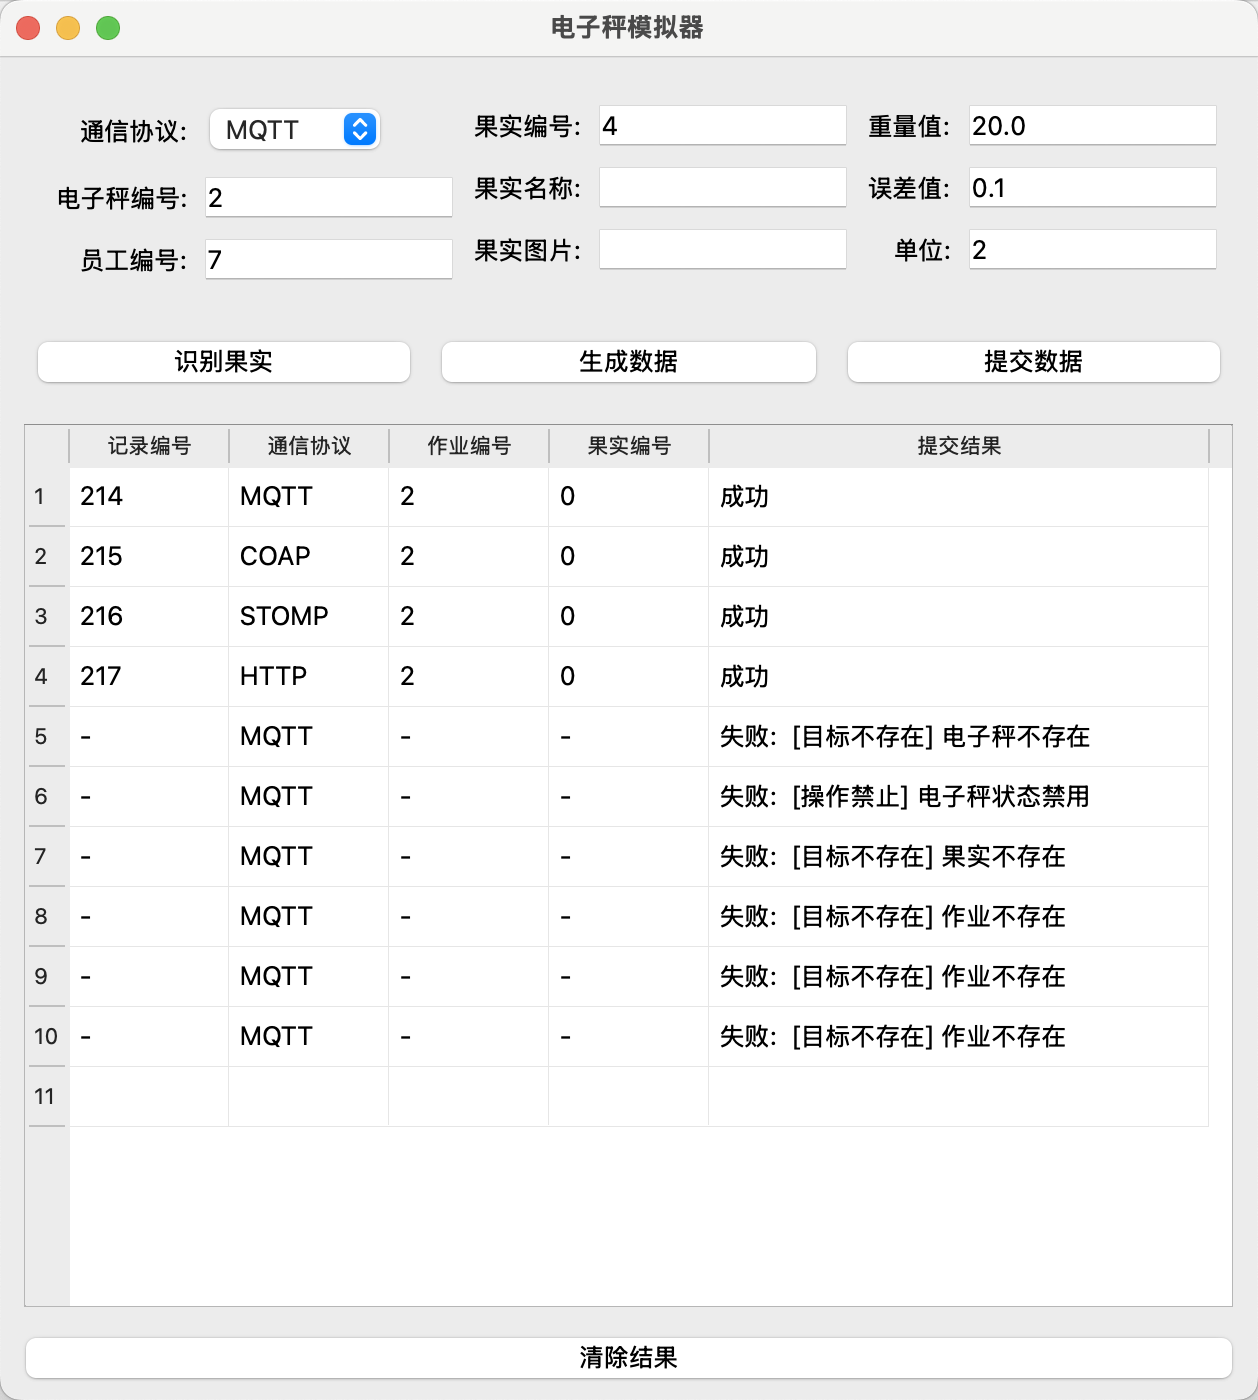
\includegraphics[width=0.8\linewidth]{../result/weigh-submit-result.png}
    \caption{提交称重数据用例测试}
    \label{fig:weigh-submit-result}
\end{figure}

对处理待办记录需求用例\ref{tab:uc-todo-handle}设计测试用例并进行测试,如表\ref{tab:uc-todo-handle-test}所示。

\begin{longtblr}
    [
    caption        = {处理待办记录测试用例},
    label          = {tab:uc-todo-handle-test}
    ]
    {
        colspec={Q[c,m]X[c,m]},
        hlines,vlines,cell{2-Z}{1}={},
        cell{1-Z}{1}={font=\bfseries},
        cell{1-Z}{2}={halign=l}
    }
用例名称 & 处理待办记录 \\

用例描述 & 管理员在管理后台界面处理待办记录 \\

用例入口 & 后台管理界面中的待办管理模块 \\

测试步骤 & 步骤1. 点击提交待办 \newline
步骤2. 选择果实种类 \newline
步骤3. 点击确定,完成待办 \\

测试用例 & 用例1: 提交正常数据 \newline
用例2: 提交异常数据(不存在的果实, 果实编号为999) \newline
用例3: 提交异常数据(未启用的果实, 果实编号为1) \\

预期结果与实际结果 & 用例1:预期返回"成功",实际结果一致 \newline
用例2:预期返回"失败",实际结果一致 \newline
用例3:预期返回"失败",实际结果一致 \\

\end{longtblr}

实际界面的测试情况如图\ref{fig:todo-handle-result-1}和图\ref{fig:todo-handle-result-2}所示。

\begin{figure}[H]
    \centering
    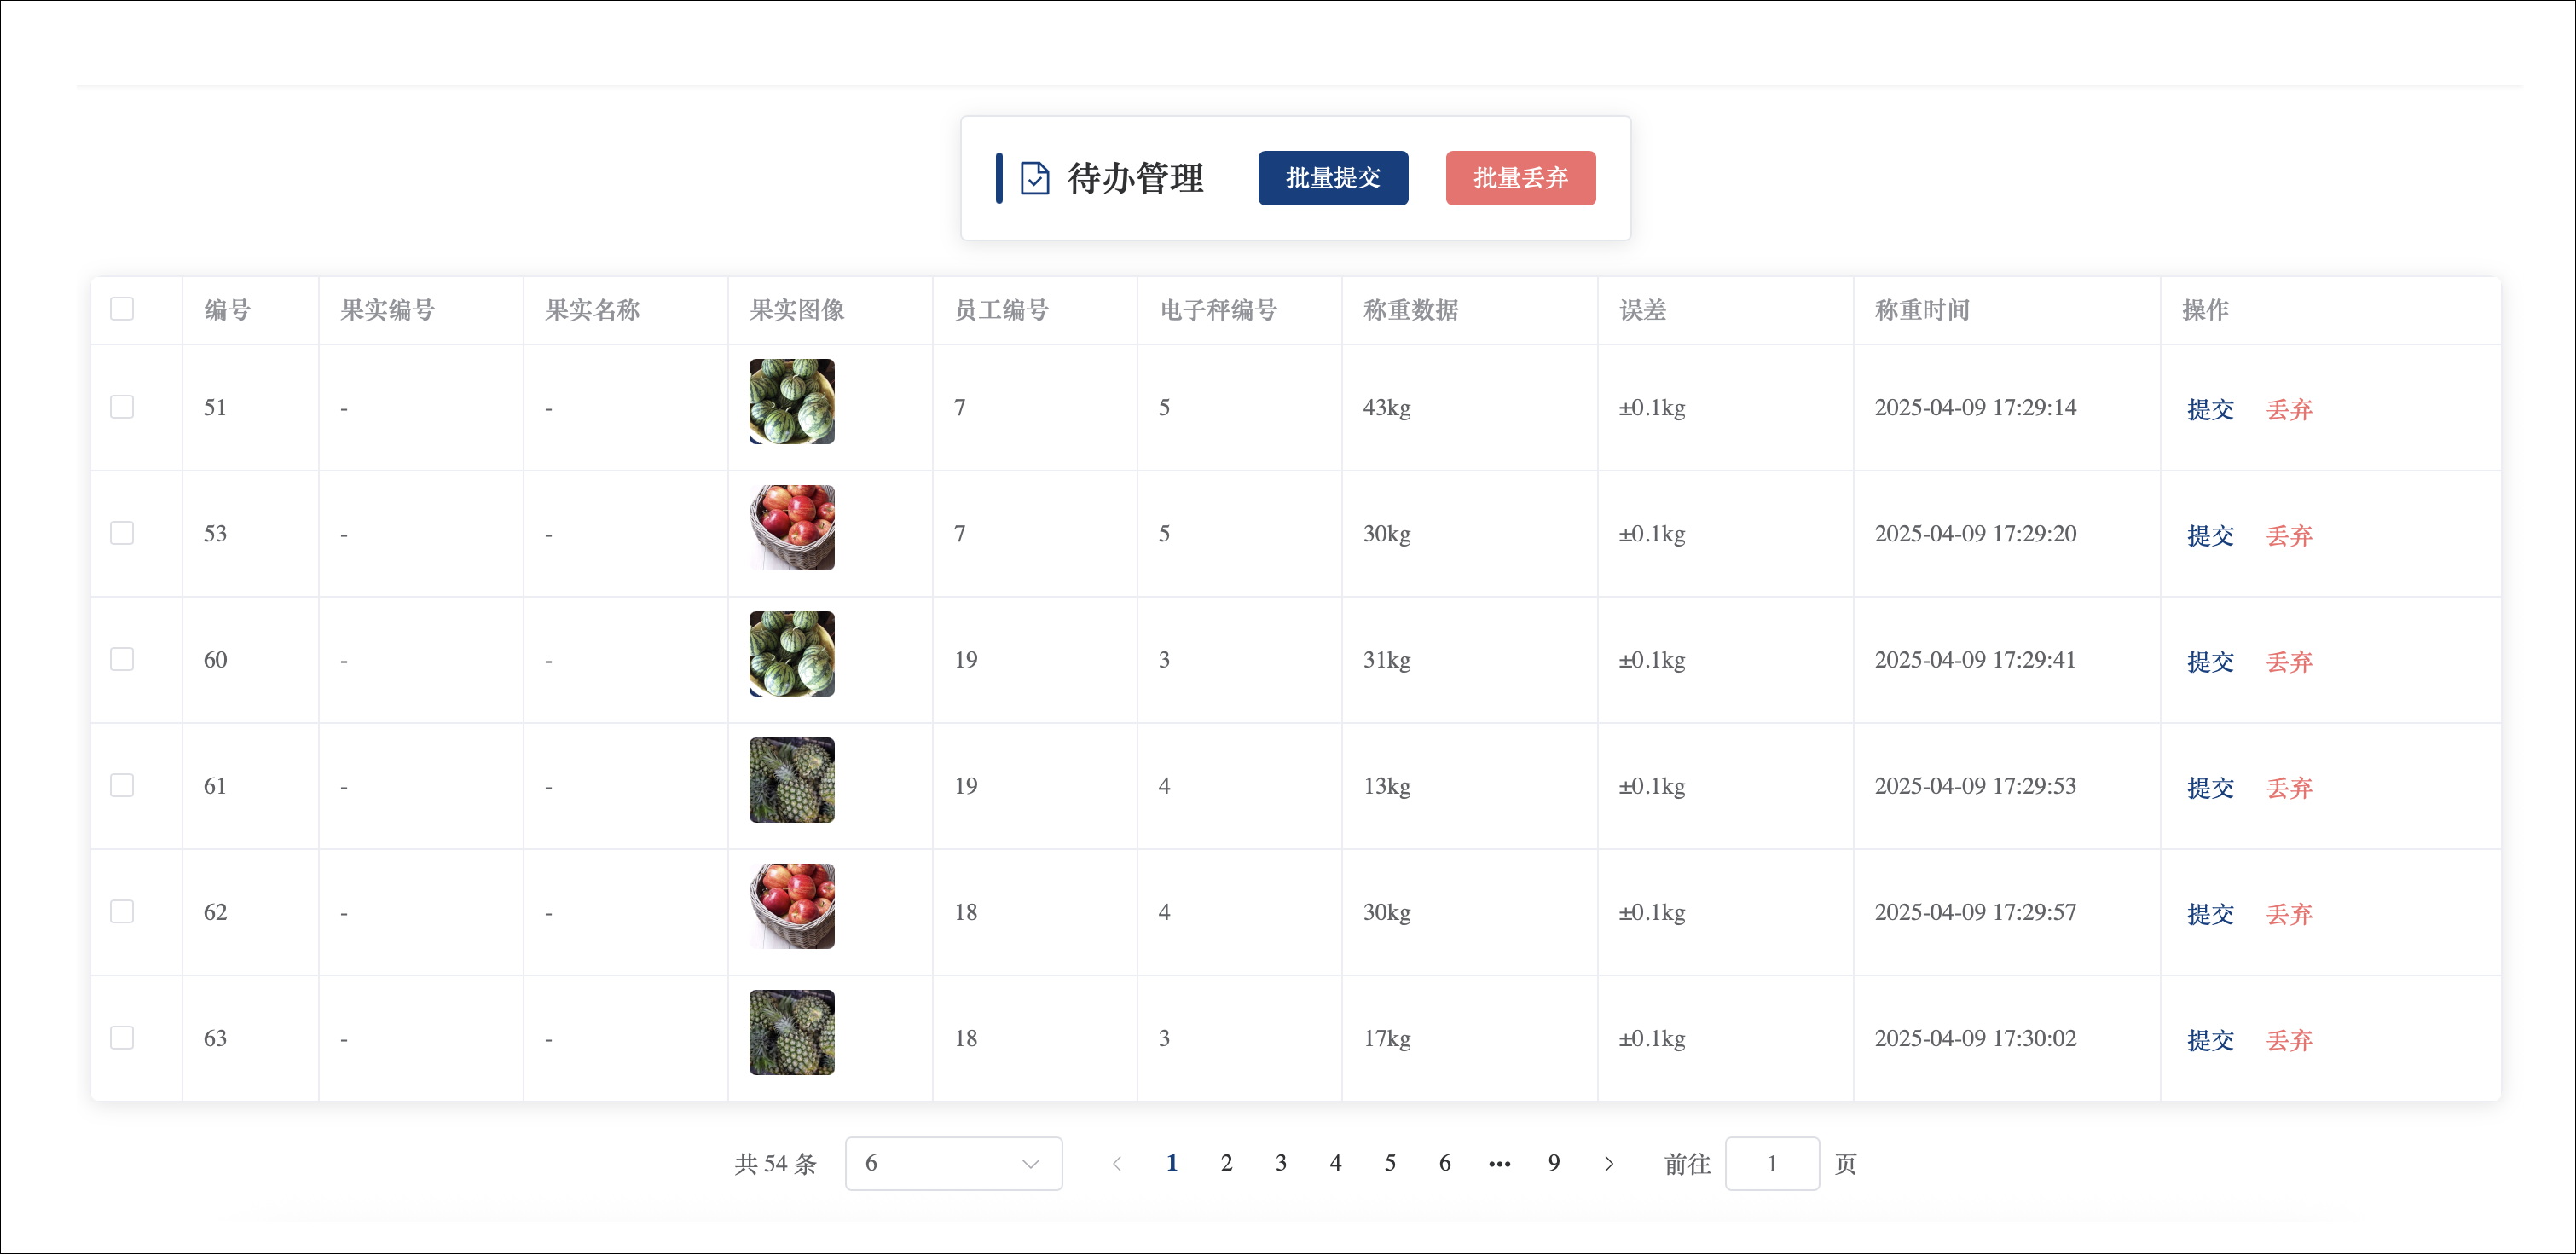
\includegraphics[width=0.95\linewidth]{../result/todo-handle-result-1.png}
    \caption{处理待办记录用例测试}
    \label{fig:todo-handle-result-1}
\end{figure}

如图\ref{fig:todo-handle-result-1}所示,展现了软件管理后台中的待办管理界面,其中包含待办列表、4个操作按钮和分页块,其中待办列表表头包含编号、果实编号、果实名称、果实图像、员工编号、电子秤编号、称重数据、误差、称重时间和操作;操作按钮包含提交、丢弃、批量提交和批量丢弃。对某个待办项,点击提交按钮后,显示表单如图\ref{fig:todo-handle-result-2}所示。

\begin{figure}[H]
    \centering
    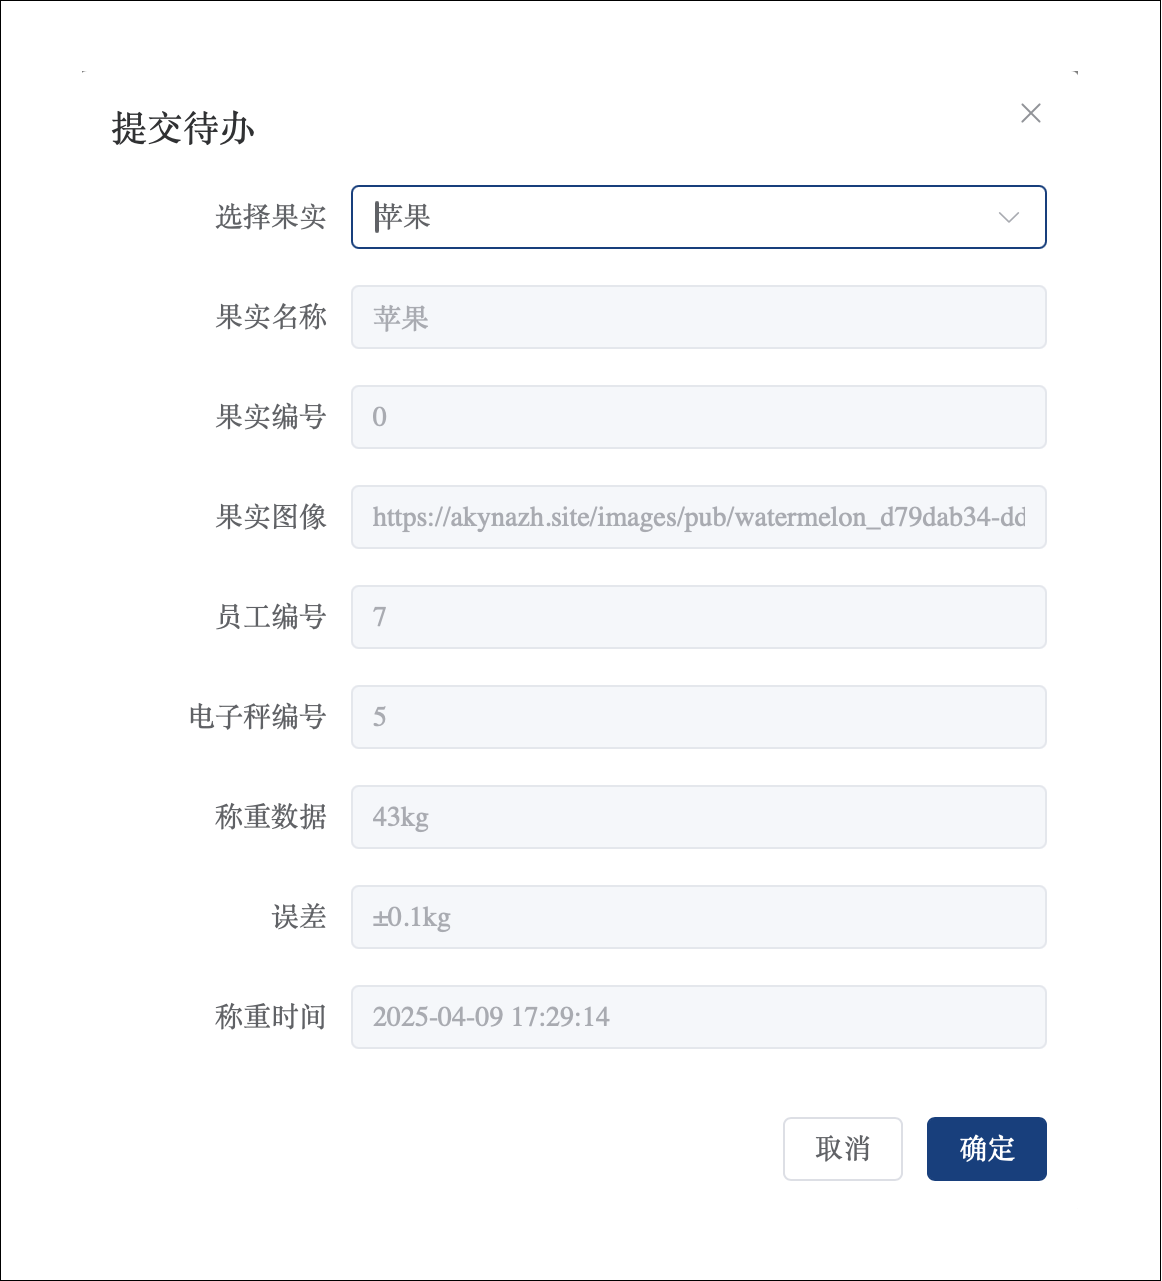
\includegraphics[width=0.8\linewidth]{../result/todo-handle-result-2.png}
    \caption{处理待办记录用例测试}
    \label{fig:todo-handle-result-2}
\end{figure}

图\ref{fig:todo-handle-result-2}展现了待办项的提交表单,包含2个操作按钮和9个表单项,其中操作按钮包含取消和确认按钮;表单项包含选择果实、果实名称、果实编号、果实图像、员工编号、电子秤编号、称重数据、误差、称重时间,其中只能编辑果实,从选择果实项的下滑表单中选择果实后,果实名称和果实编号项将会随之变化。

对称重记录统计分析需求用例\ref{tab:uc-record-analysis}设计测试用例并进行测试,如表\ref{tab:uc-record-analysis-test}所示。

\begin{longtblr}
    [
    caption        = {称重记录统计分析测试用例},
    label          = {tab:uc-record-analysis-test}
    ]
    {
        colspec={Q[c,m]X[c,m]},
        hlines,vlines,cell{2-Z}{1}={},
        cell{1-Z}{1}={font=\bfseries},
        cell{1-Z}{2}={halign=l}
    }

用例名称 & 称重记录统计分析 \\

用例描述 & 在管理后台界面查看果实和采摘人员的称重记录统计情况 \\

用例入口 & 后台管理界面中的果实/用户管理模块 \\

测试步骤 & 步骤1. 管理员访问果实/用户管理界面 \newline
步骤2. 管理员点击某个可视化选项进行查看并导出 \\

测试用例 & 用例1:点击查看苹果的年产量并导出为 Excel \newline
用例2: 点击查看苹果的分批产量并导出为 Excel \newline
用例3: 点击查看用户(用户编号为3)的分批产量并导出为 Excel  \\

预期结果与实际结果 & 用例1:预期得到折线图和对应的 Excel 表格,实际结果一致 \newline
用例2:预期得到折线图和对应的 Excel 表格,实际结果一致 \newline
用例3:预期得到折线图和对应的 Excel 表格,实际结果一致 \\

\end{longtblr}

实际界面的测试情况如图\ref{fig:record-analysis-result-1}和图\ref{fig:record-analysis-result-2}所示。

\begin{figure}[H]
    \centering
    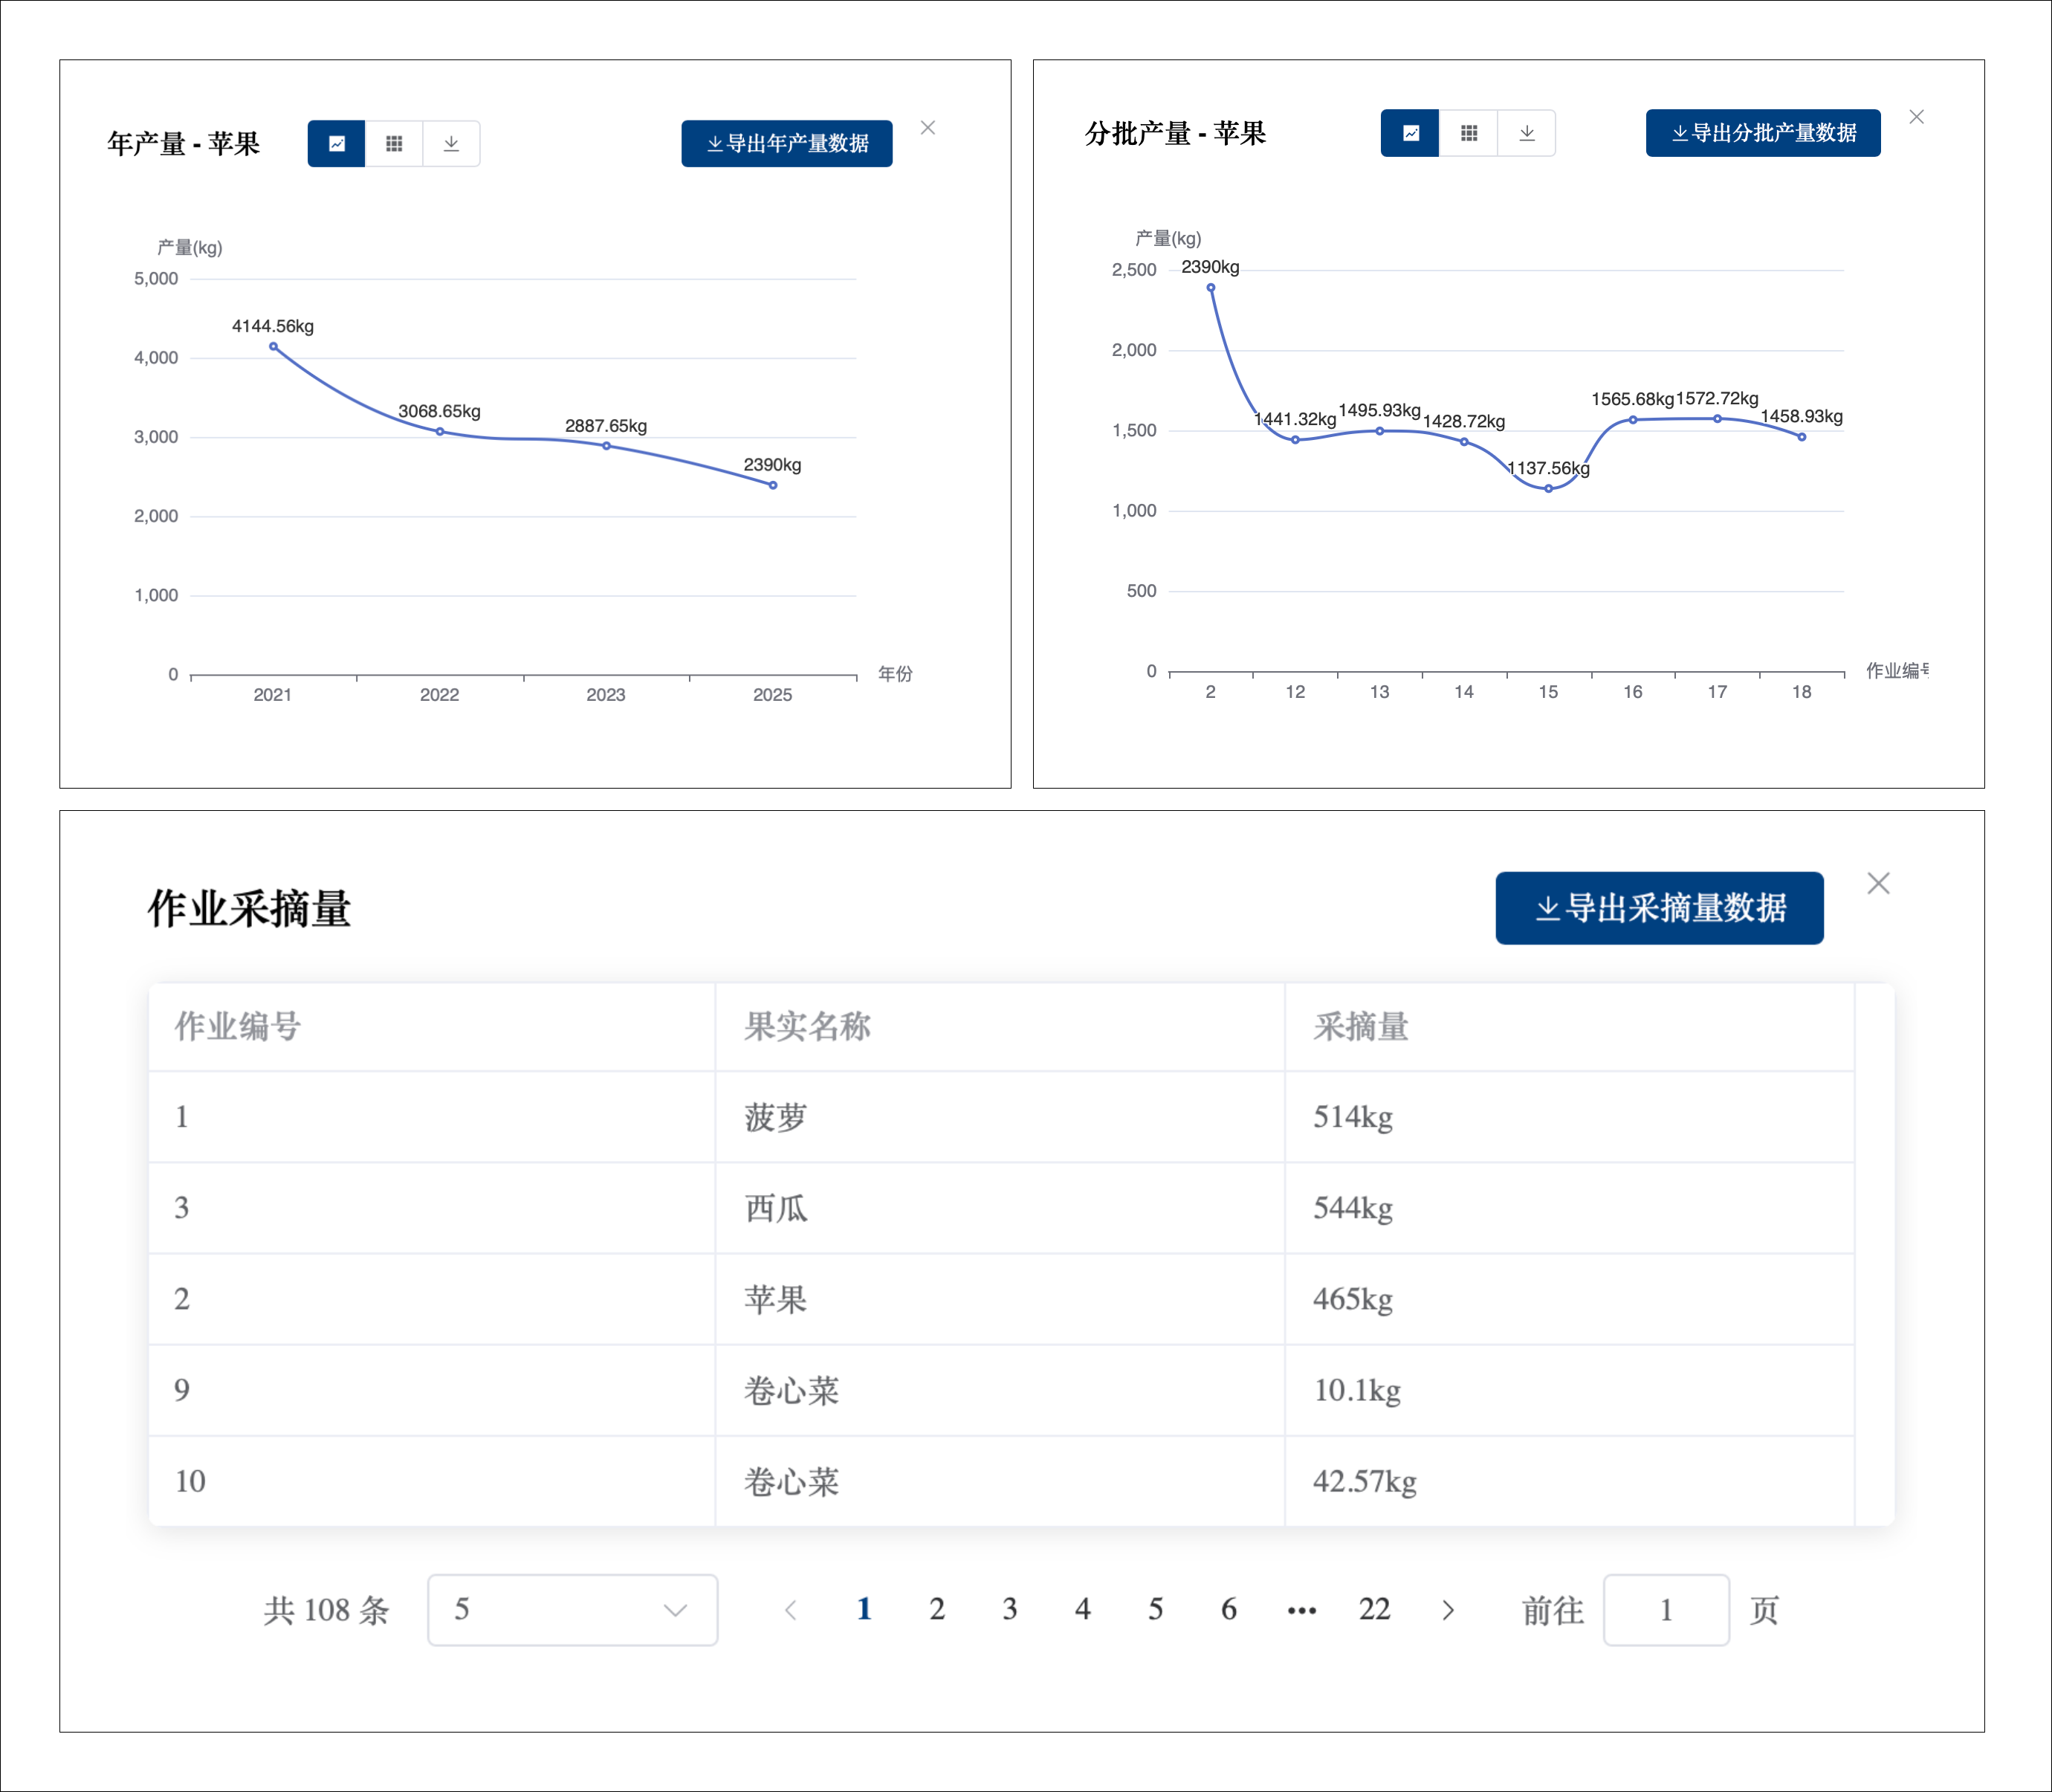
\includegraphics[width=0.9\linewidth]{../result/record-analysis-result-1.png}
    \caption{称重记录统计分析用例测试}
    \label{fig:record-analysis-result-1}
\end{figure}

如图\ref{fig:record-analysis-result-1}所示,上方两个折线图展现了果实的年产量和分批产量,下方的表格展现了用户的分批采摘量情况。其中果实的年产量折线图中,横坐标为年份,纵坐标为产量(kg);果实的分批产量折线图中,横坐标为作业编号,纵坐标为产量(kg);用户分批采摘量表格中,表头包含作业编号、果实名称和采摘量。

每个可视化图表都支持导出,点击图表右上方的导出按钮即可完成 Excel 导出,导出情况如图\ref{fig:record-analysis-result-2}所示。

\begin{figure}[H]
    \centering
    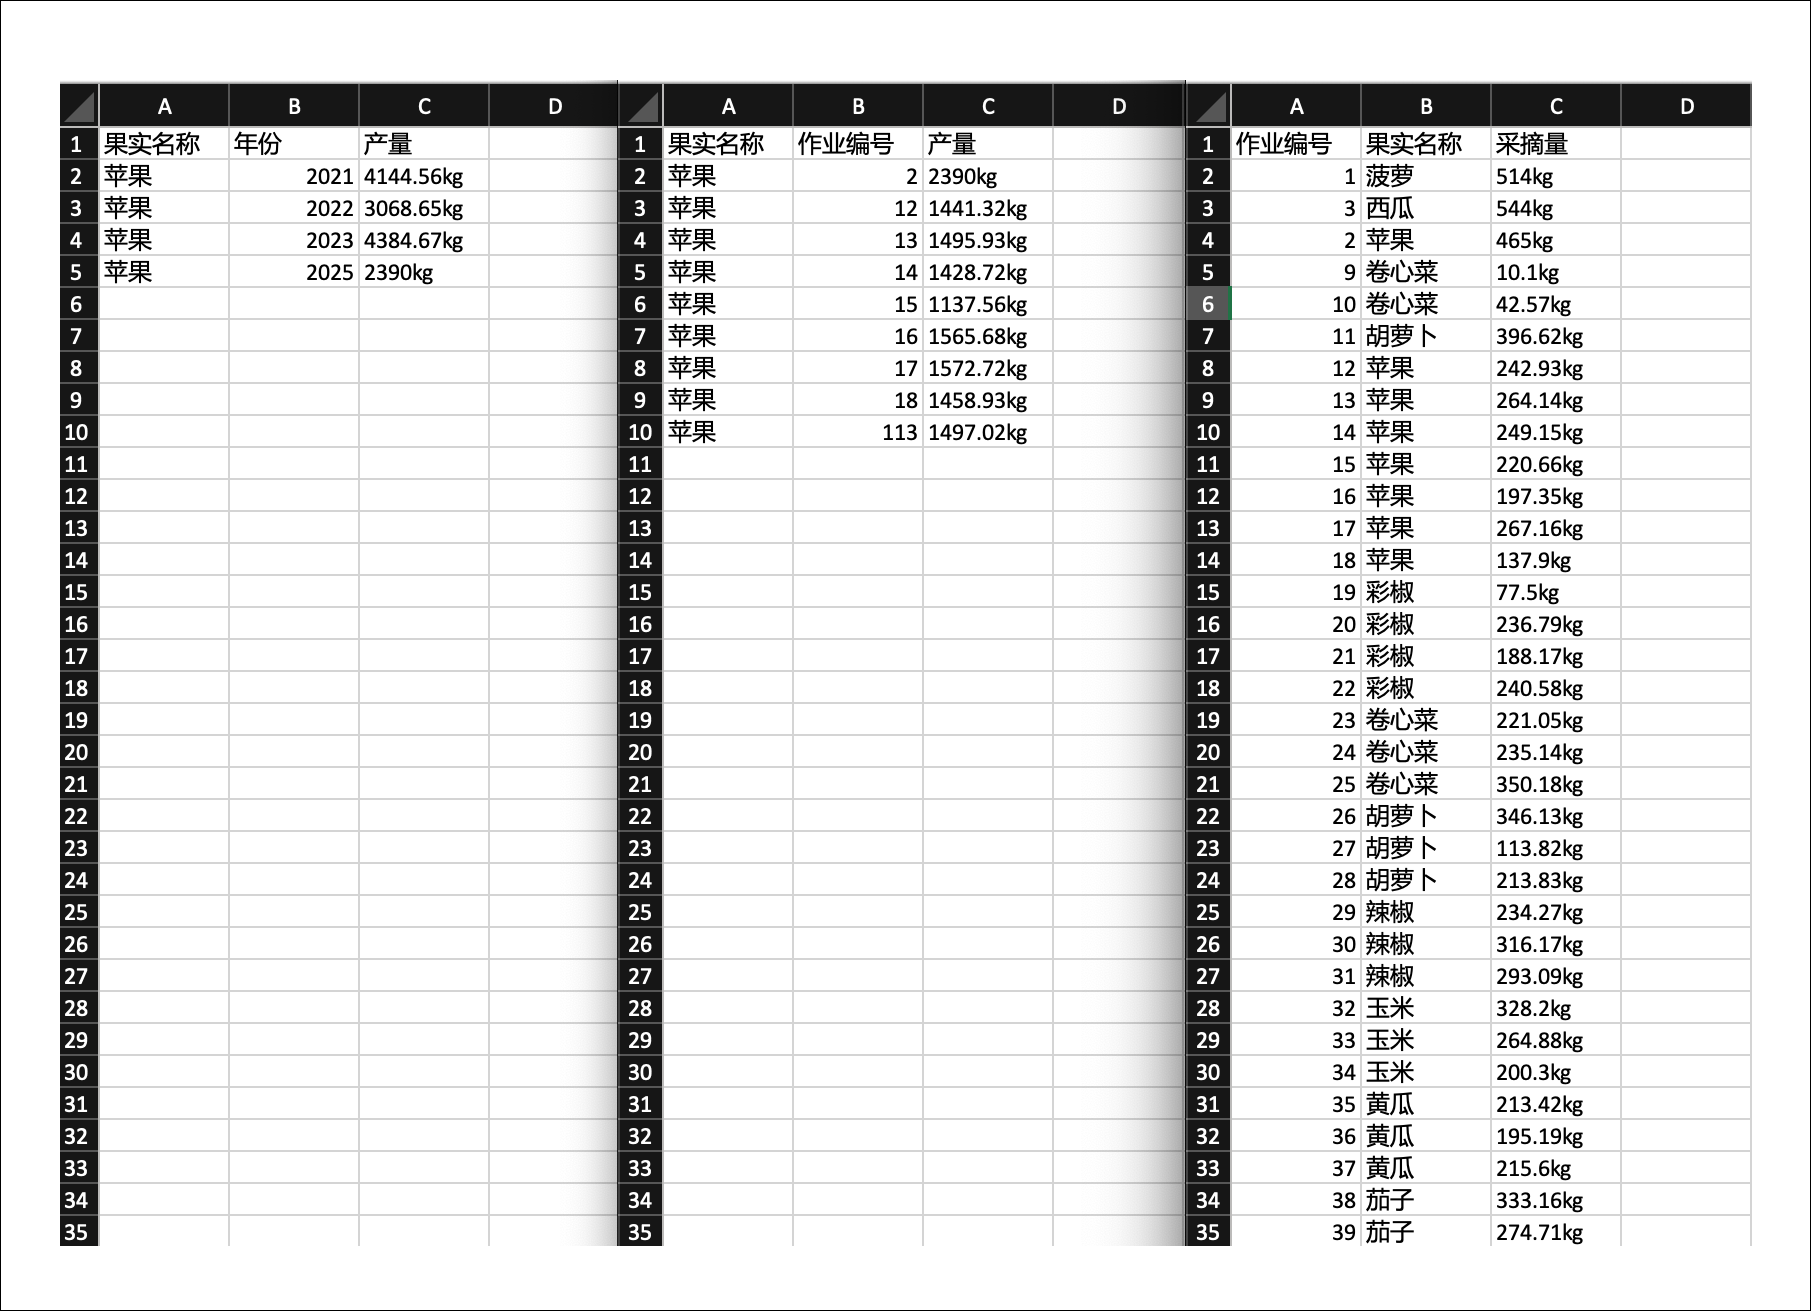
\includegraphics[width=0.9\linewidth]{../result/record-analysis-result-2.png}
    \caption{称重记录统计分析用例测试}
    \label{fig:record-analysis-result-2}
\end{figure}

如图\ref{fig:record-analysis-result-2}所示,从左至右分别展现了果实的年产量表格、果实的分批产量表格和用户的分批采摘量表格。

对用户认证和授权需求用例\ref{tab:uc-user-auth}设计测试用例并进行测试,如表\ref{tab:uc-user-auth-test}所示。

\begin{longtblr}
    [
    caption        = {用户认证和授权测试用例},
    label          = {tab:uc-user-auth-test}
    ]
    {
        colspec={Q[c,m]X[c,m]},
        hlines,vlines,cell{2-Z}{1}={},
        cell{1-Z}{1}={font=\bfseries},
        cell{1-Z}{2}={halign=l}
    }

用例名称 & 用户认证和授权 \\

用例描述 & 用户在后台管理界面中执行操作时的认证和授权流程 \\

用例入口 & 接口请求工具 Rest Client \\

测试步骤 & 步骤1. 调用登录接口获取到认证令牌 \newline
步骤2. 调用普通用户功能接口 \newline
步骤3. 调用管理员功能接口 \\

测试用例 & 用例1:采摘员工调用查看个人信息接口 \newline
用例2: 管理员调用查看个人信息接口 \newline
用例3: 采摘员工调用查看用户列表接口 \newline
用例4: 管理员调用查看用户列表接口 \\

预期结果与实际结果 & 用例1:预期返回数据和状态码 200,实际结果一致 \newline
用例2:预期返回数据和状态码 200,实际结果一致 \newline
用例3:预期返回错误信息和状态码 403,实际结果一致 \newline
用例4:预期返回数据和状态码 200,实际结果一致 \\
\end{longtblr}

实际界面的测试情况如图\ref{fig:user-auth-admin}和\ref{fig:user-auth-emp}所示。

\begin{figure}[H]
    \centering
    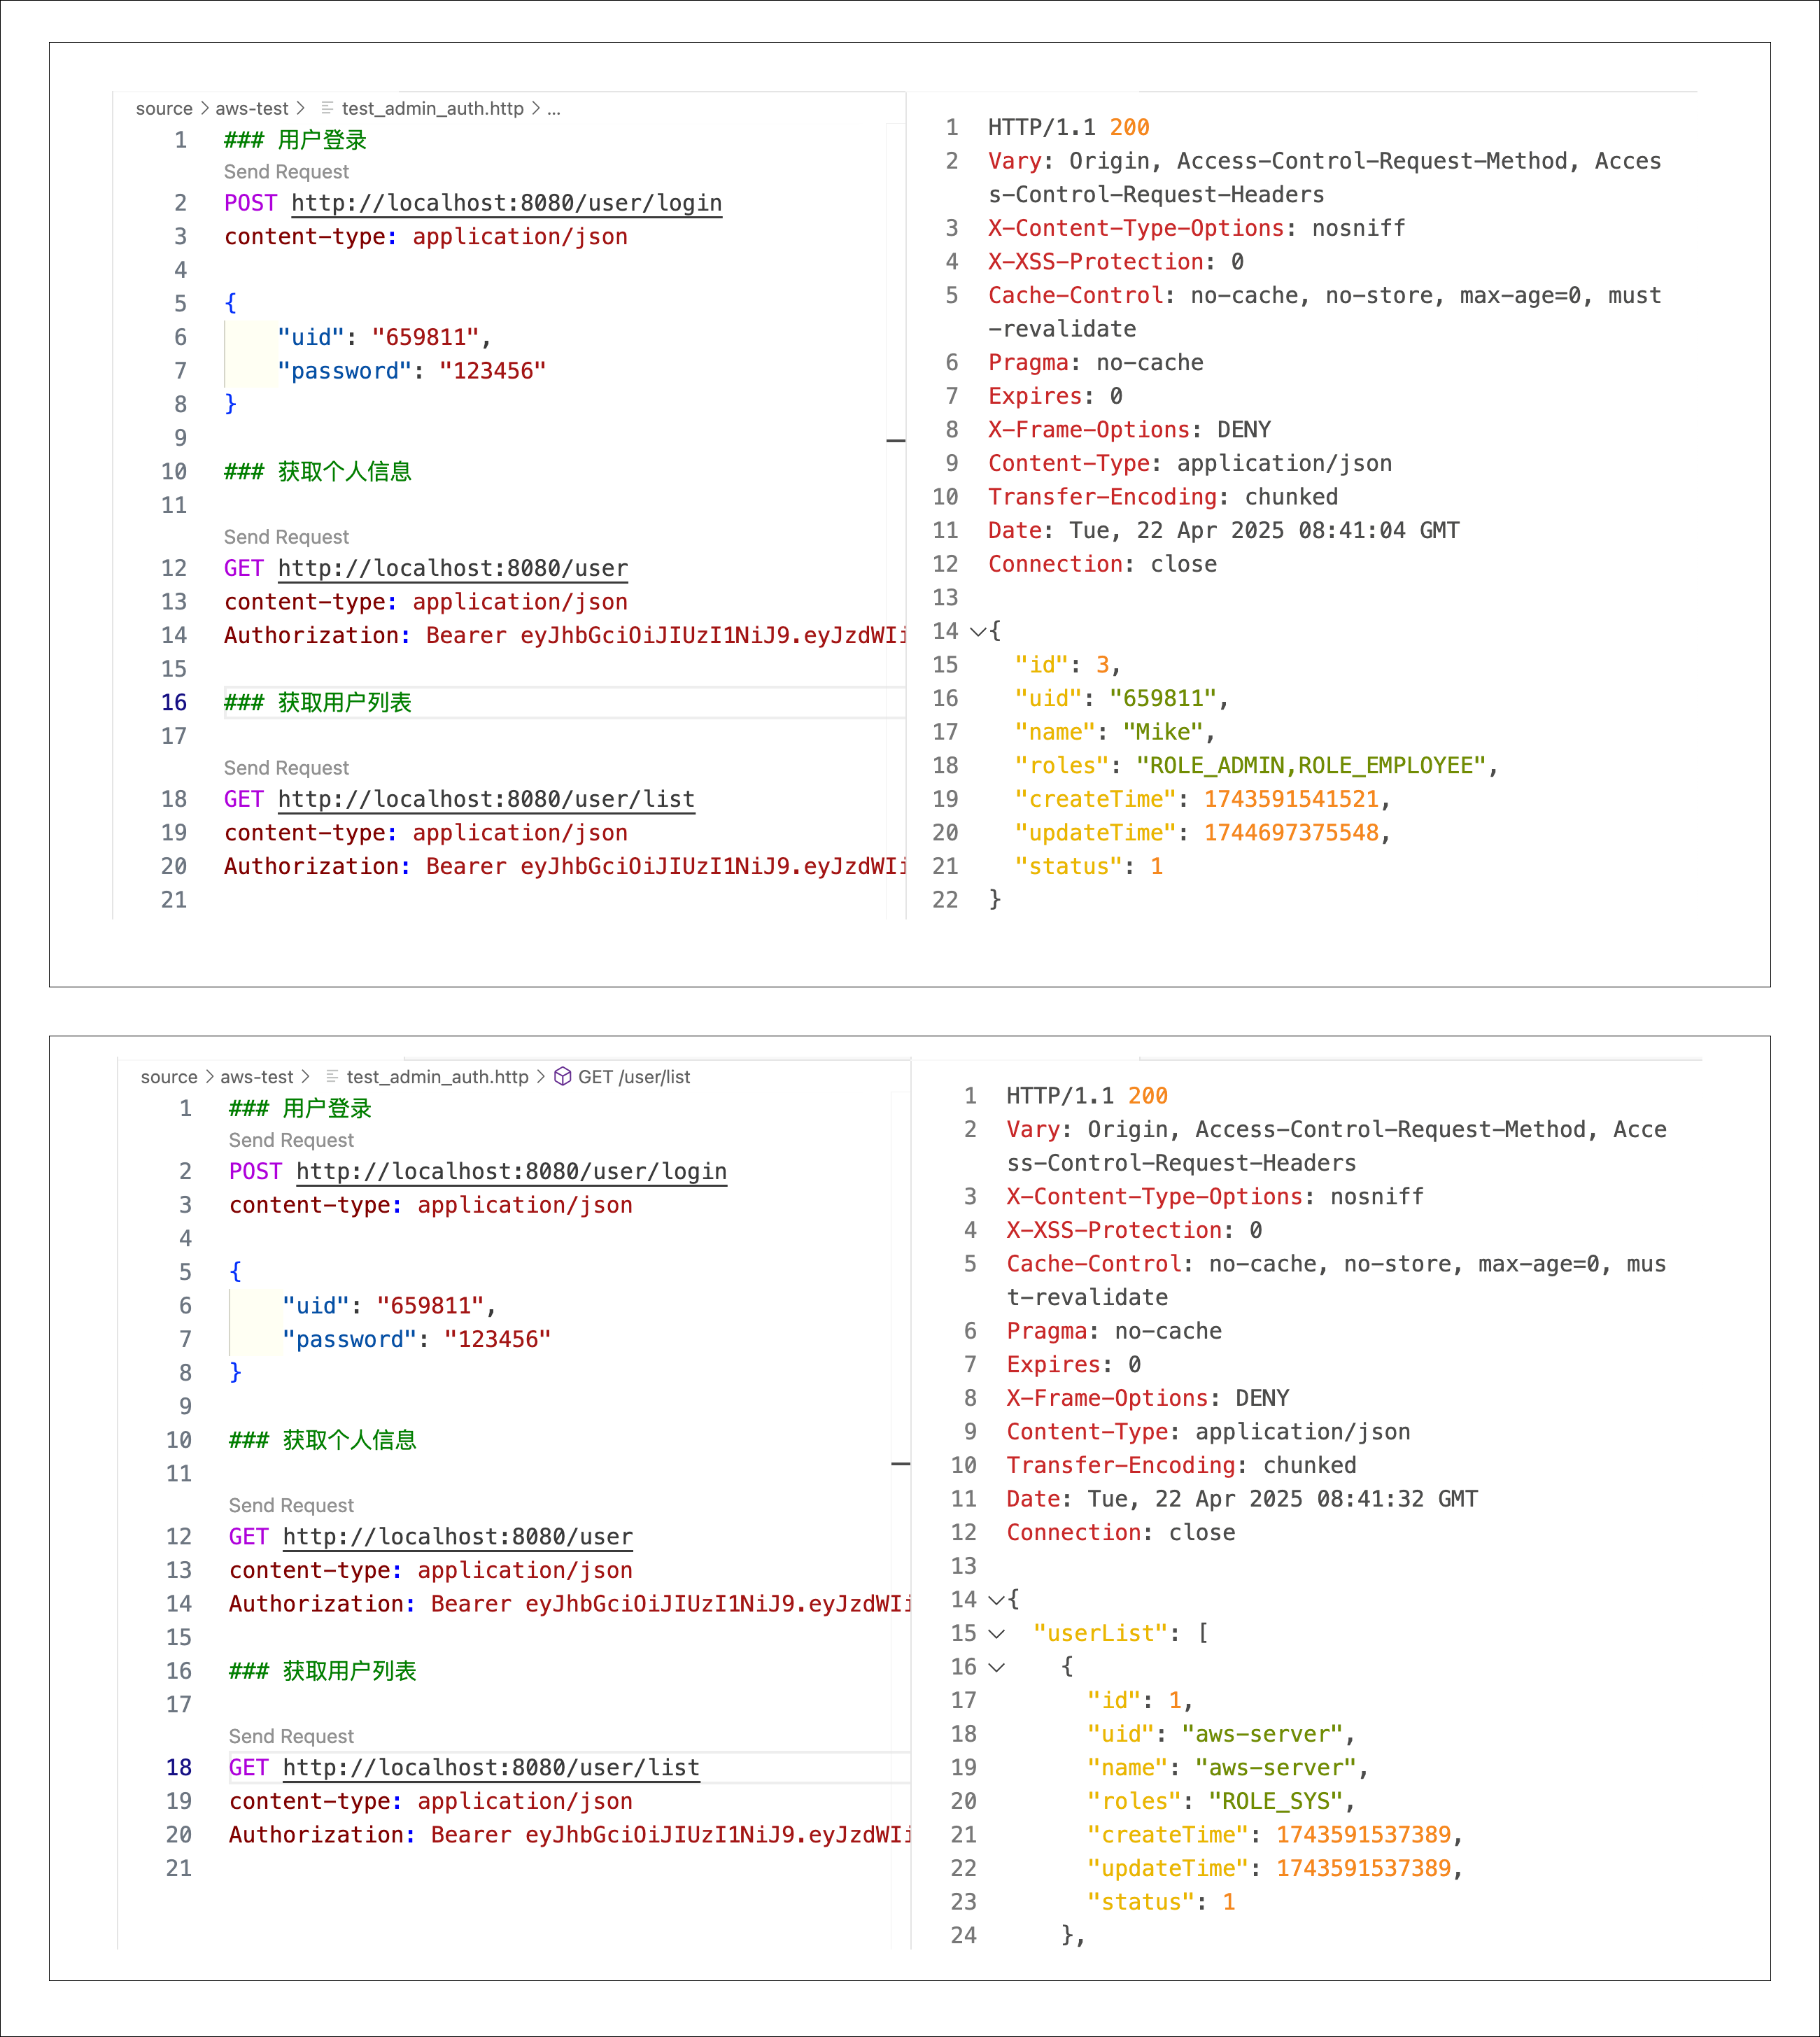
\includegraphics[width=0.9\linewidth]{../result/user-auth-admin.png}
    \caption{管理员认证和授权用例测试}
    \label{fig:user-auth-admin}
\end{figure}

图\ref{fig:user-auth-admin}展现了管理员调用接口的结果。首先调用用户登录接口获取到认证令牌;接着通过令牌调用查看个人信息接口,返回个人信息,其中用户角色显示为管理员(ROLE\_ADMIN),状态码为 200;最后调用查看用户列表接口,返回用户列表,状态码为200。结果符合预期,测试通过。

\begin{figure}[H]
    \centering
    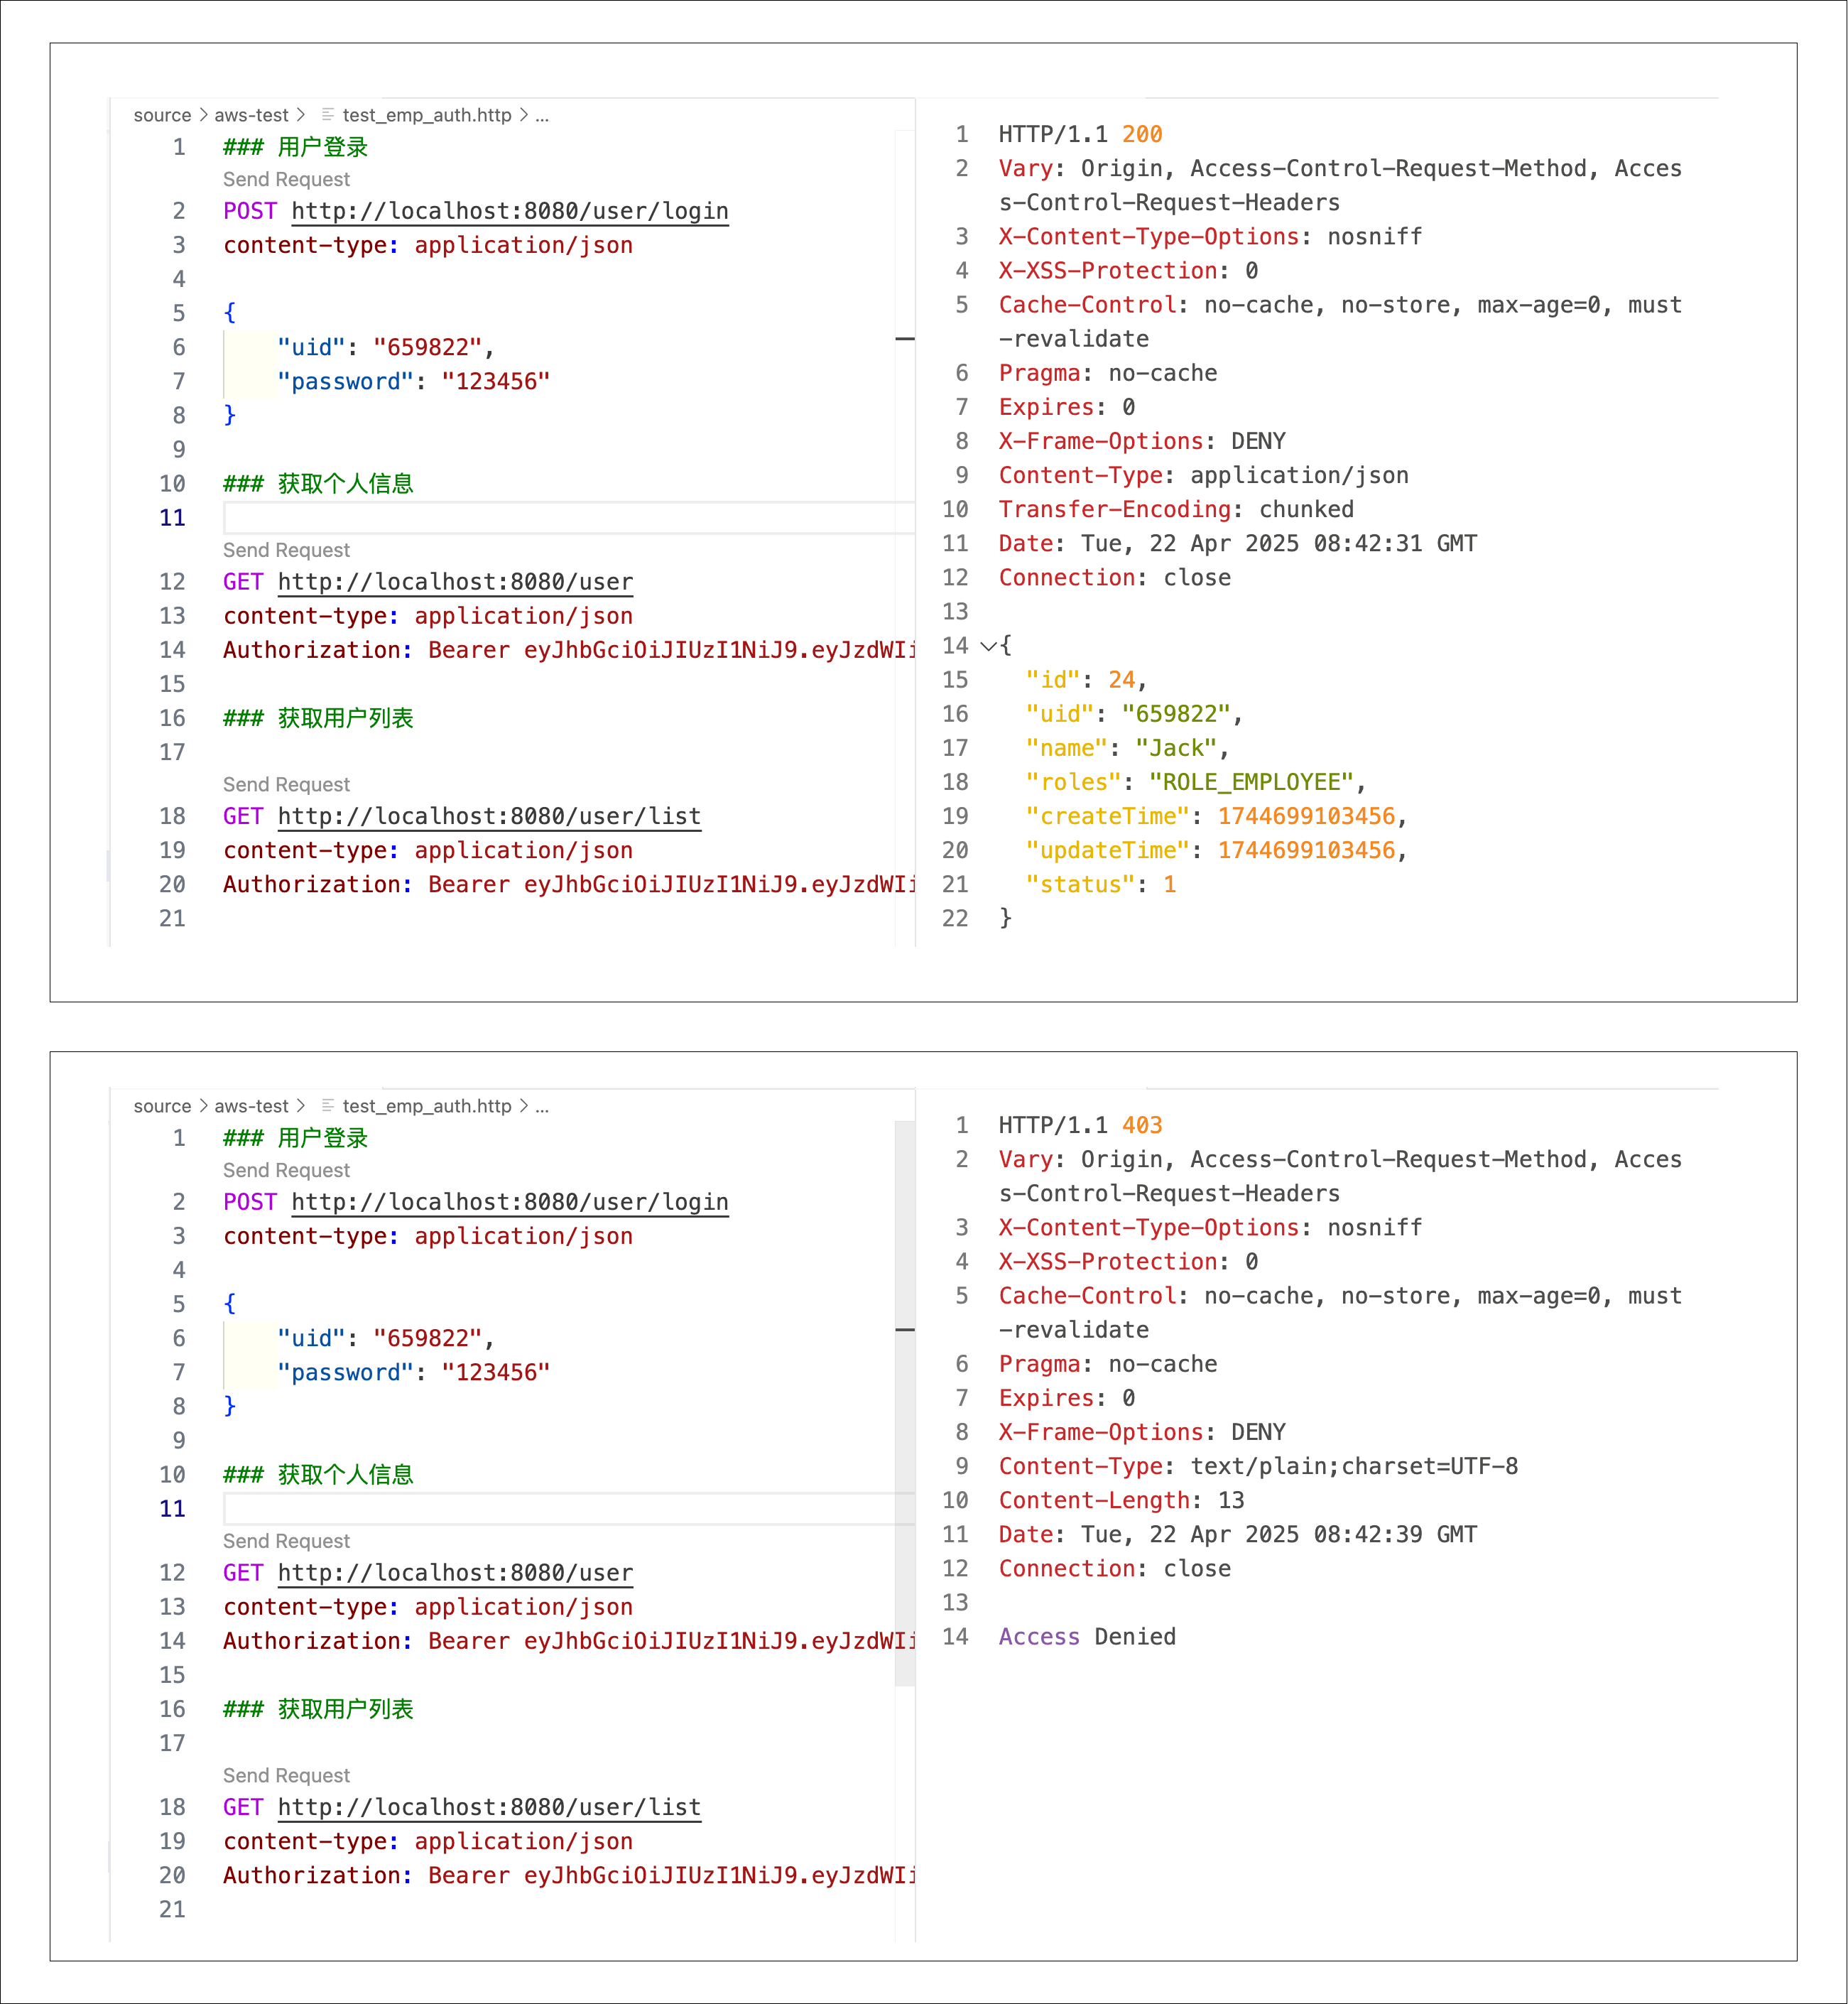
\includegraphics[width=0.9\linewidth]{../result/user-auth-emp.png}
    \caption{采摘员工认证和授权用例测试}
    \label{fig:user-auth-emp}
\end{figure}

图\ref{fig:user-auth-admin}展现了采摘员工调用接口的结果。首先调用用户登录接口获取到认证令牌;接着通过令牌调用查看个人信息接口,返回个人信息,其中用户角色显示为采摘员工(ROLE\_EMPLOYEE),状态码为 200;最后调用查看用户列表接口,返回 Access Denied(访问拒绝),状态码为 403。结果符合预期,测试通过。

\newpage
对果实图像识别需求用例\ref{tab:uc-produce-predict}设计测试用例并进行测试,如表\ref{tab:uc-produce-predict-test}所示。

\begin{longtblr}
    [
    caption        = {果实图像识别测试用例},
    label          = {tab:uc-produce-predict-test}
    ]
    {
        colspec={Q[c,m]X[c,m]},
        hlines,vlines,cell{2-Z}{1}={},
        cell{1-Z}{1}={font=\bfseries},
        cell{1-Z}{2}={halign=l}
    }
用例名称 & 果实图像识别用例 \\

用例描述 & 调用本地模型推理预测果实种类 \\

用例入口 & 接口请求工具 Rest Client \\

测试步骤 & 步骤1. 输入果实图片地址 \newline
步骤2. 调用果实图像识别接口 \\

测试用例 & 用例1:提交模型支持的果实图片(苹果) \newline
用例2: 提交模型不支持的果实图片(火龙果) \\

预期结果与实际结果 & 用例1:预期为成功预测果实种类为苹果且置信度高于 0.8,实际结果一致 \newline
用例2:预期为错误预测果实种类且置信度低于 0.8,实际结果一致 \\

\end{longtblr}

实际界面的测试情况如图\ref{fig:produce-predict}所示。

\begin{figure}[H]
    \centering
    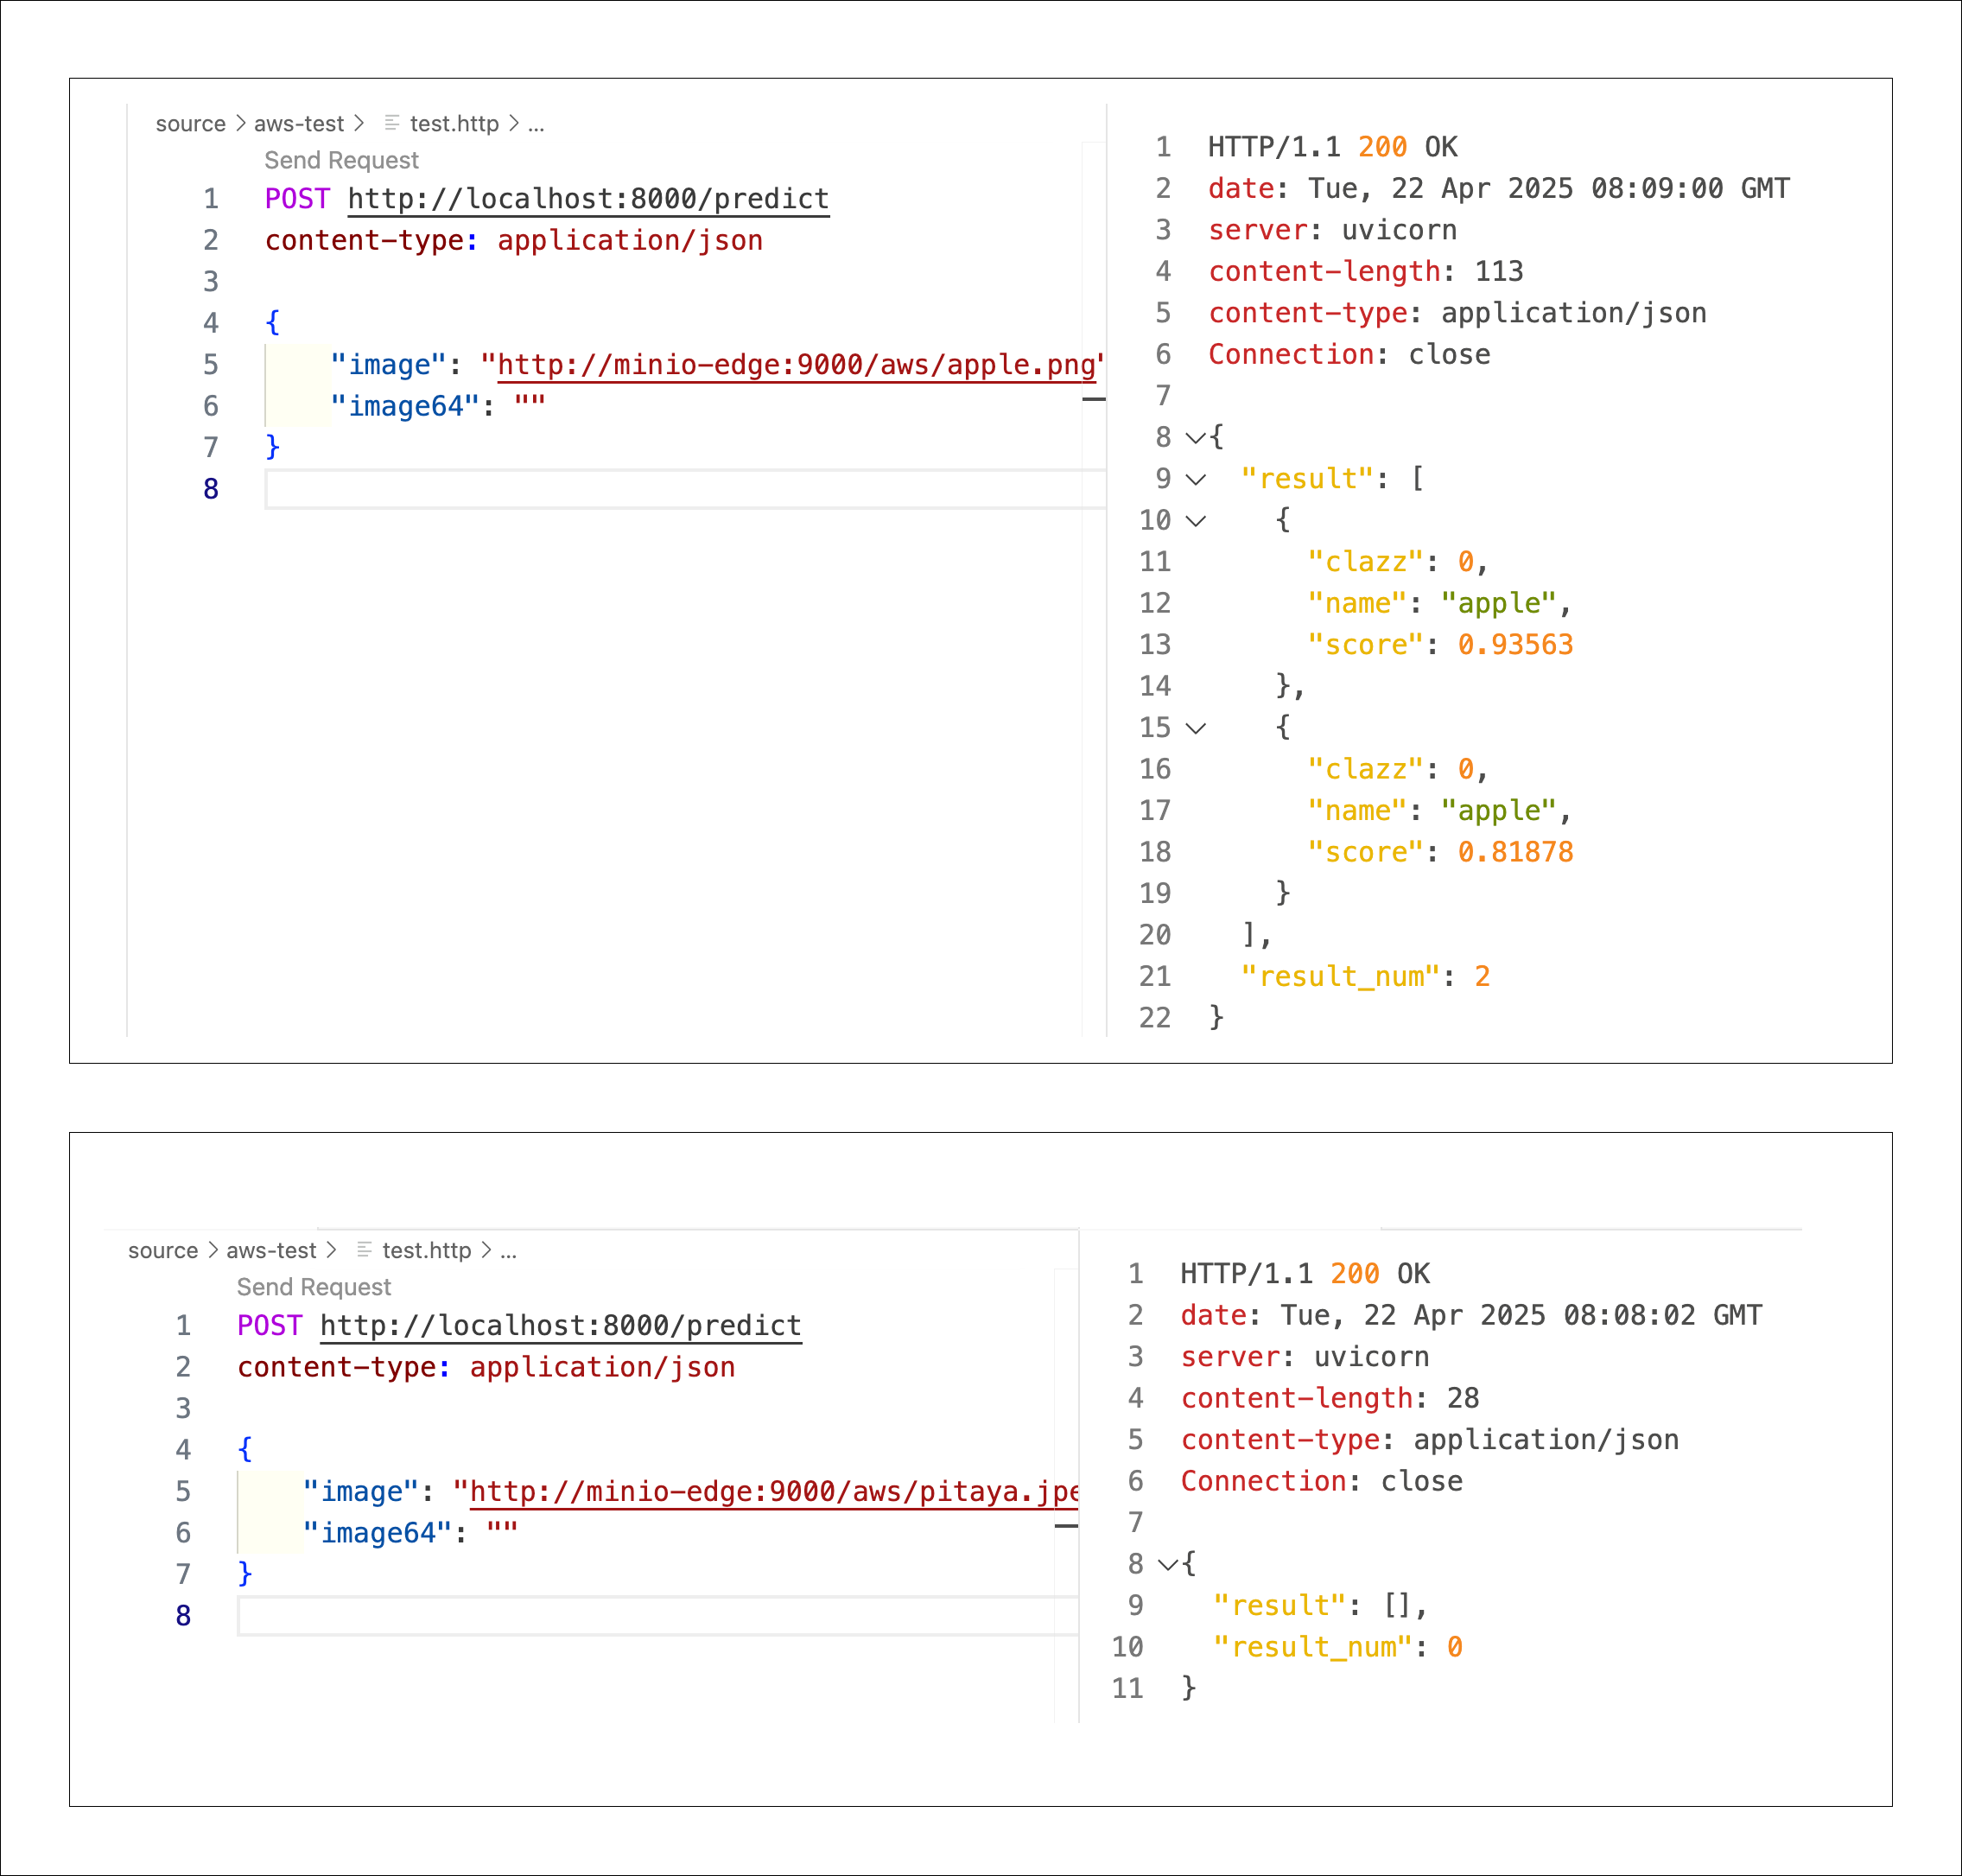
\includegraphics[width=0.9\linewidth]{../result/produce-predict.png}
    \caption{果实图像识别用例测试}
    \label{fig:produce-predict}
\end{figure}

如图\ref{fig:produce-predict}所示,图中上方请求提交了苹果图片,返回结果中得到预测置信度排名第一位的果实为苹果,置信度为 0.93563,符合预期;下方请求显示提交了火龙果图片,返回结果为空,预测失败,符合预期。

对新建采摘作业需求用例\ref{tab:uc-work-new}设计测试用例并进行测试,如表\ref{tab:uc-work-new-test}所示。

\begin{longtblr}
    [
    caption        = {新建采摘作业测试用例},
    label          = {tab:uc-work-new-test}
    ]
    {
        colspec={Q[c,m]X[c,m]},
        hlines,vlines,cell{2-Z}{1}={},
        cell{1-Z}{1}={font=\bfseries},
        cell{1-Z}{2}={halign=l}
    }

用例名称 & 新建采摘作业用例 \\

用例描述 & 对某一果实新建对于采摘作业 \\

用例入口 & 后台管理界面中的作业管理模块 \\

测试步骤 & 步骤1. 点击添加作业 \newline
步骤2. 选择采摘产品 \newline
步骤3. 选择起止时间 \newline
步骤4. 点击确认完成添加 \\

测试用例 & 用例1: 提交正常数据(选择已启用的果实:苹果) \newline
用例2: 提交异常数据(选择未启用的果实:香蕉) \newline
用例3: 提交异常数据(选择已有对应采摘作业的果实:苹果) \\

预期结果与实际结果 & 用例1:预期返回"成功",实际结果一致 \newline
用例2:预期返回"失败",实际结果一致 \newline
用例3:预期返回"失败",实际结果一致 \\

\end{longtblr}

实际界面的测试情况如图\ref{fig:work-new-result-1}和图\ref{fig:work-new-result-2}所示。

\begin{figure}[H]
    \centering
    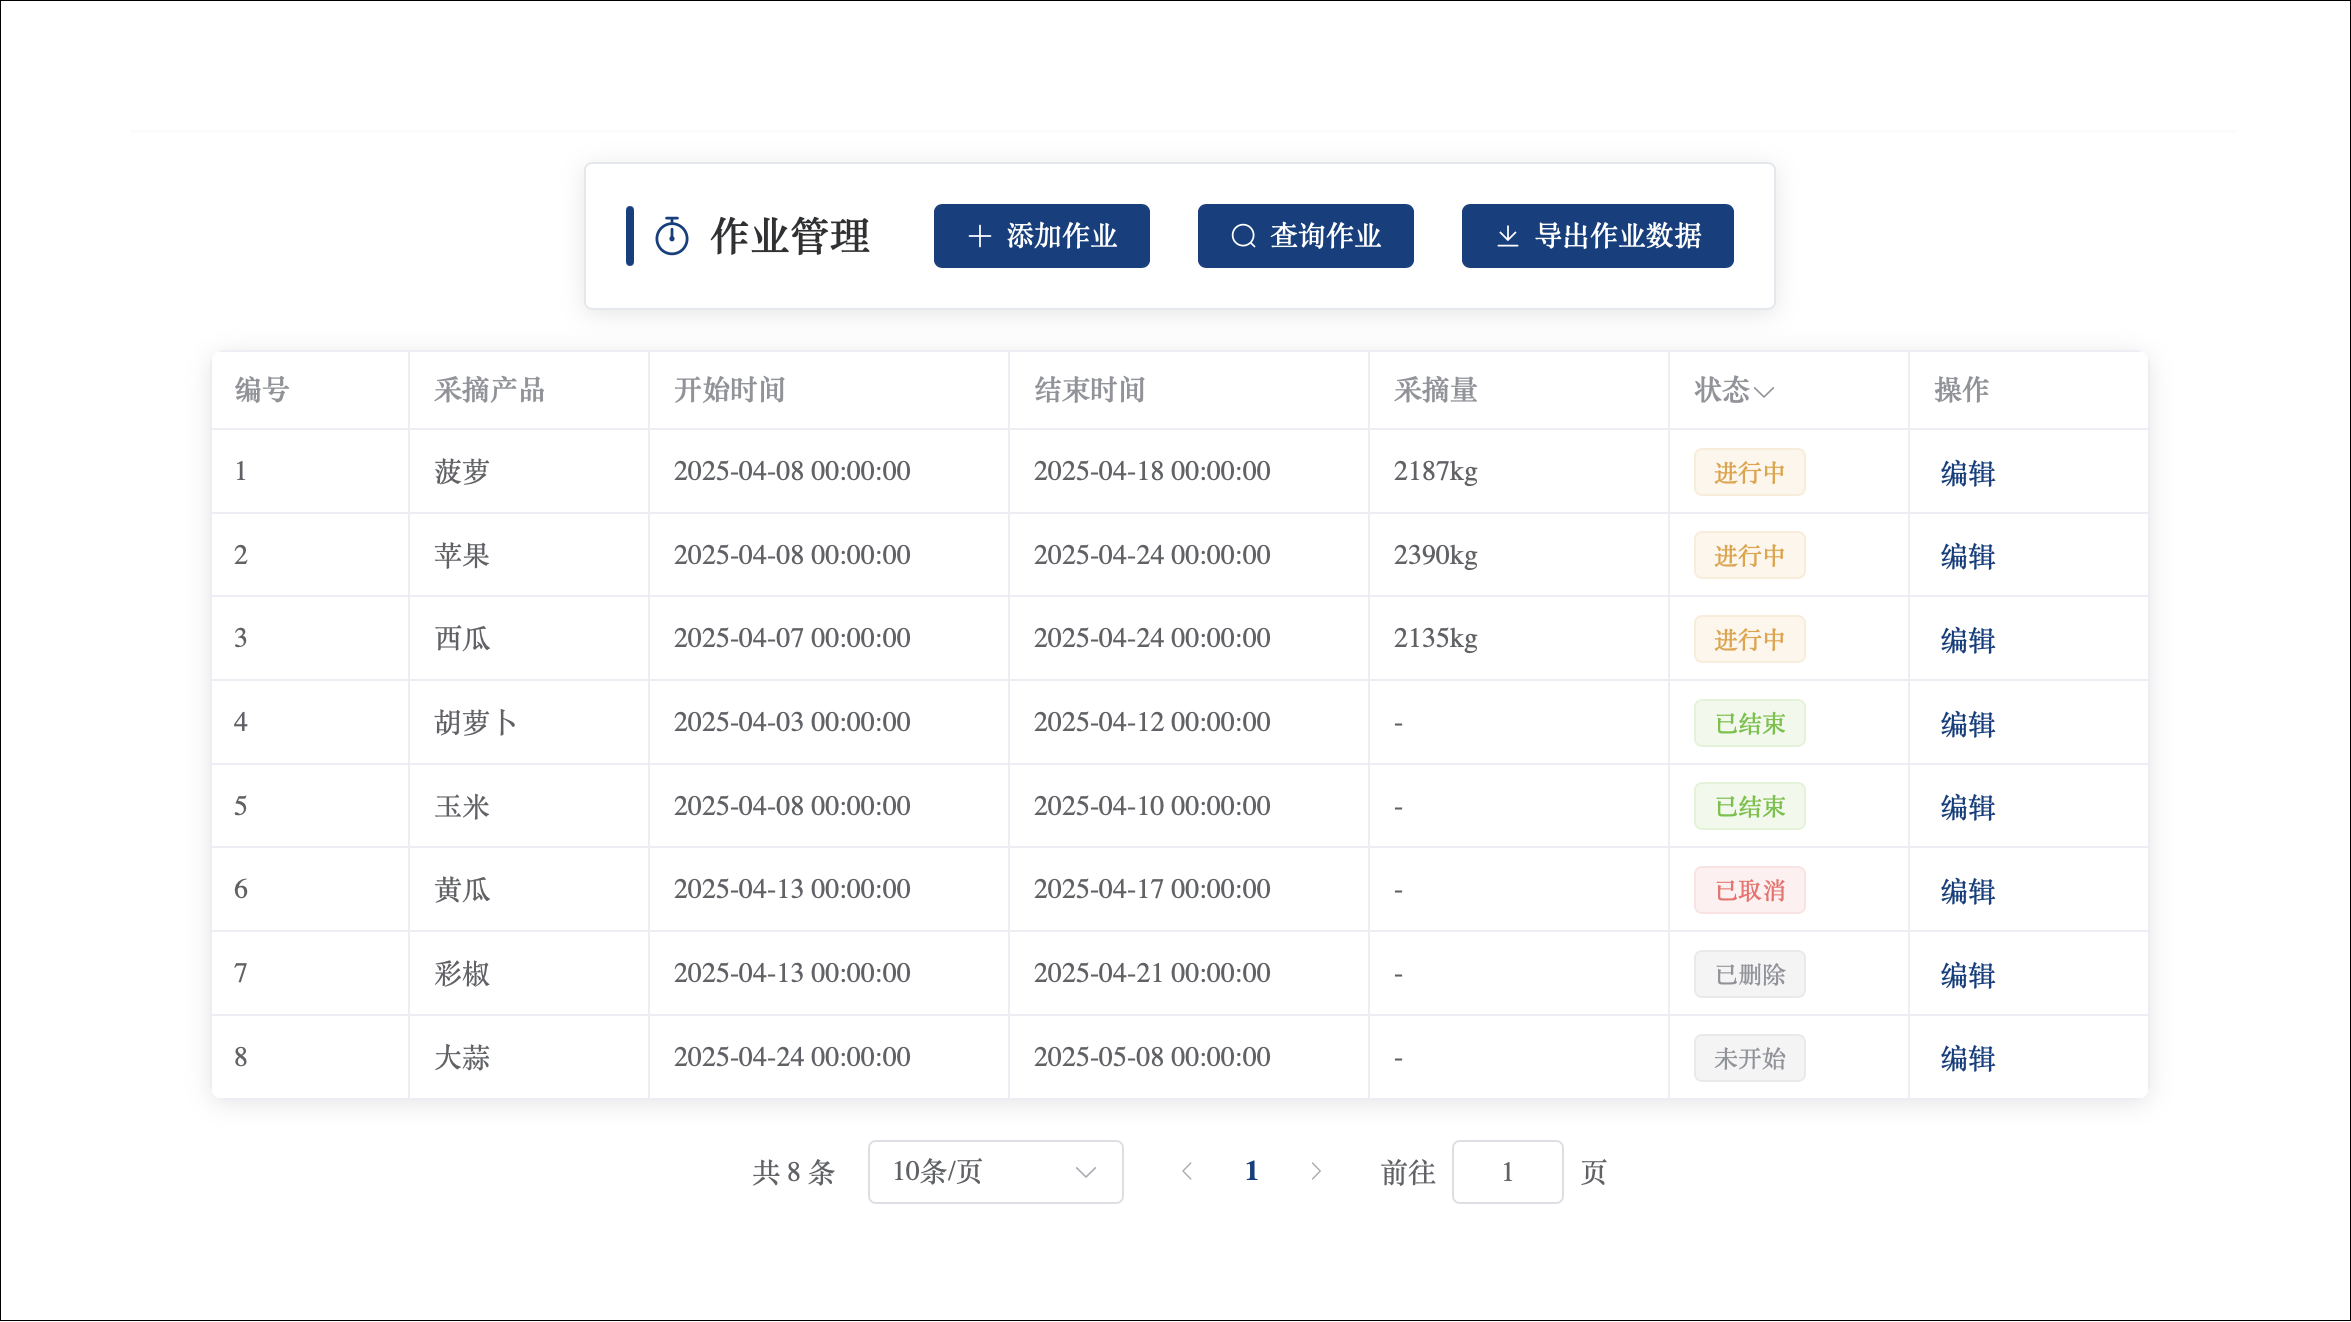
\includegraphics[width=0.9\linewidth]{../result/work-new-result-1.png}
    \caption{新建采摘作业用例测试}
    \label{fig:work-new-result-1}
\end{figure}

如图\ref{fig:work-new-result-1}所示,展现了软件管理后台中的作业管理界面,其中包含作业列表、4个操作按钮和分页块,其中作业列表表头包含编号、采摘产品、开始时间、结束时间、采摘量、状态和操作;操作按钮包含添加作业、查询作业、导出作业数据和编辑。点击添加作业按钮后,显示表单如图\ref{fig:work-new-result-2}所示。

\begin{figure}[H]
    \centering
    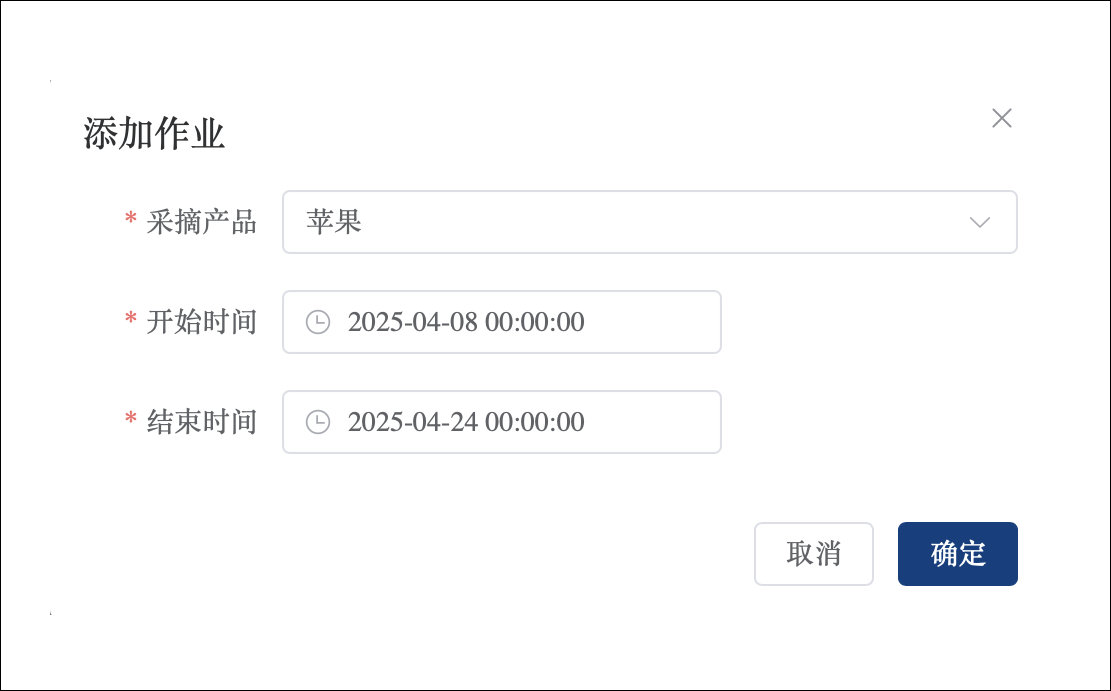
\includegraphics[width=0.8\linewidth]{../result/work-new-result-2.png}
    \caption{新建采摘作业用例测试}
    \label{fig:work-new-result-2}
\end{figure}

图\ref{fig:work-new-result-2}展现了作业项的提交表单,包含2个操作按钮和3个表单项,其中操作按钮包含取消和确认按钮;表单项包含选择采摘产品、开始时间和结束时间,采摘产品在下滑表单中选择,开始时间和结束时间点击后在日历组件中选择。

至此,完成对核心功能需求用例的测试。

\section{软件性能测试}

根据非功能需求汇总表\ref{tab:n-req-summary}中提到的功能,给出对应的实现结果,如表\ref{tab:test-n-req-summary}所示。

\begin{longtblr}
    [
    caption        = {非功能需求实现结果},
    label          = {tab:test-n-req-summary}
    ]
    {
    colspec        = {Q[c,m]X[l,m]},
    hline{1,Z}     = {wd=.08em},
    hline{2}       = {wd=.05em},
    row{even[2-Z]} = {bg=gray9!50},
    row{1}         = {font=\bfseries},
    rowhead        = 1,
    }
测试项 & 描述 & 测试结果 \\
支持多种协议 & 支持 MQTT、HTTP、CoAP、STOMP 四种协议 & 验证通过 \\
支持多种提交方式 & 支持通过果实图像/名称/编号提交称重数据 & 验证通过 \\
支持模拟提交流程 & 支持通过电子秤模拟器模拟数据提交 & 验证通过 \\
支持受限网络环境 & 支持在边端提交数据 & 验证通过 \\
提供高性能的服务 & 提供高性能的果实图像识别服务和称重数据提交服务 & 验证通过 \\
提供安全性保障 & 数据库加密敏感字段,所有接口提供认证授权保护 & 验证通过 \\
\end{longtblr}

针对提供高性能服务这个非功能需求,下面给出具体的测试和分析结果。首先给出对果实图像识别服务的性能测试,然后再给出称重数据提交服务的性能测试。

下面对训练出来的果实图像识别模型进行性能测试。

1、测试环境:4 核 CPU, 31.4GB 内存, 2 个 Tesla T4 GPU。

2、测试方式:使用 Ultralytics 提供的性能测试库,调用训练出来的最佳模型 best.pt,测试数据则采用训练集数据。

3、测试结果:如图 \ref{fig:model-benchmark} 所示。

\begin{figure}[H]
    \centering
    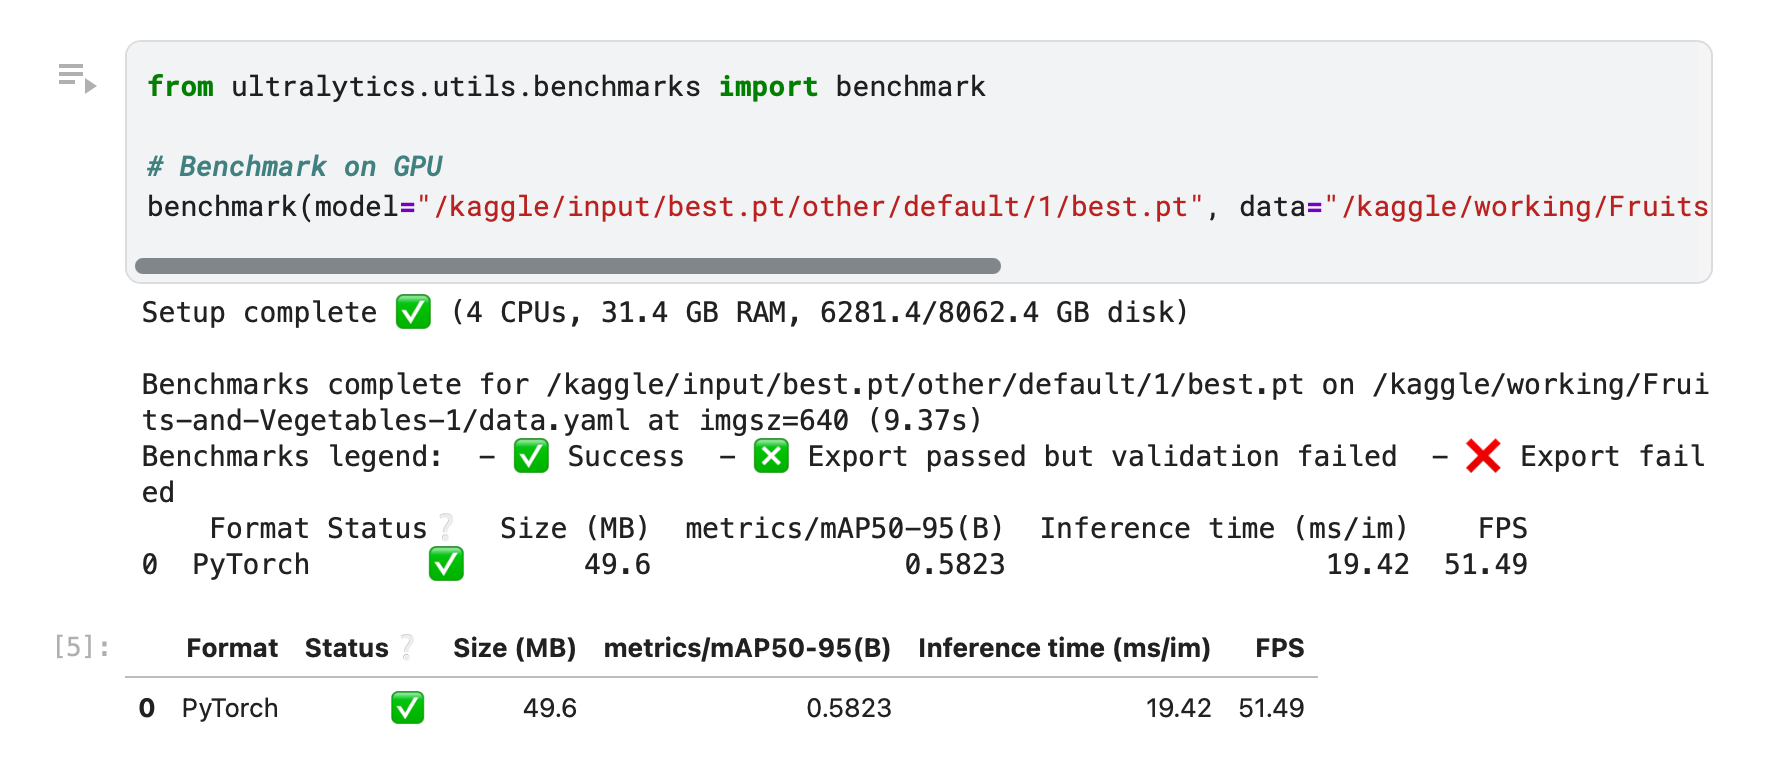
\includegraphics[width=0.8\linewidth]{../source/aws-img/yolov8/benchmark.png}
    \caption{果实图像识别模型性能测试结果}
    \label{fig:model-benchmark}
\end{figure}

从图 \ref{fig:model-benchmark} 可以得出,模型使用 PyTorch 框架训练,推理时间为 19.42 毫秒,帧率为 51.49 FPS,且在 mAP50-95 指标下的得分为 0.5823,适用于精度和推理速度之间的平衡。

此外,训练模型得到的标准化混淆矩阵图如下:

\begin{figure}[H]
    \centering
    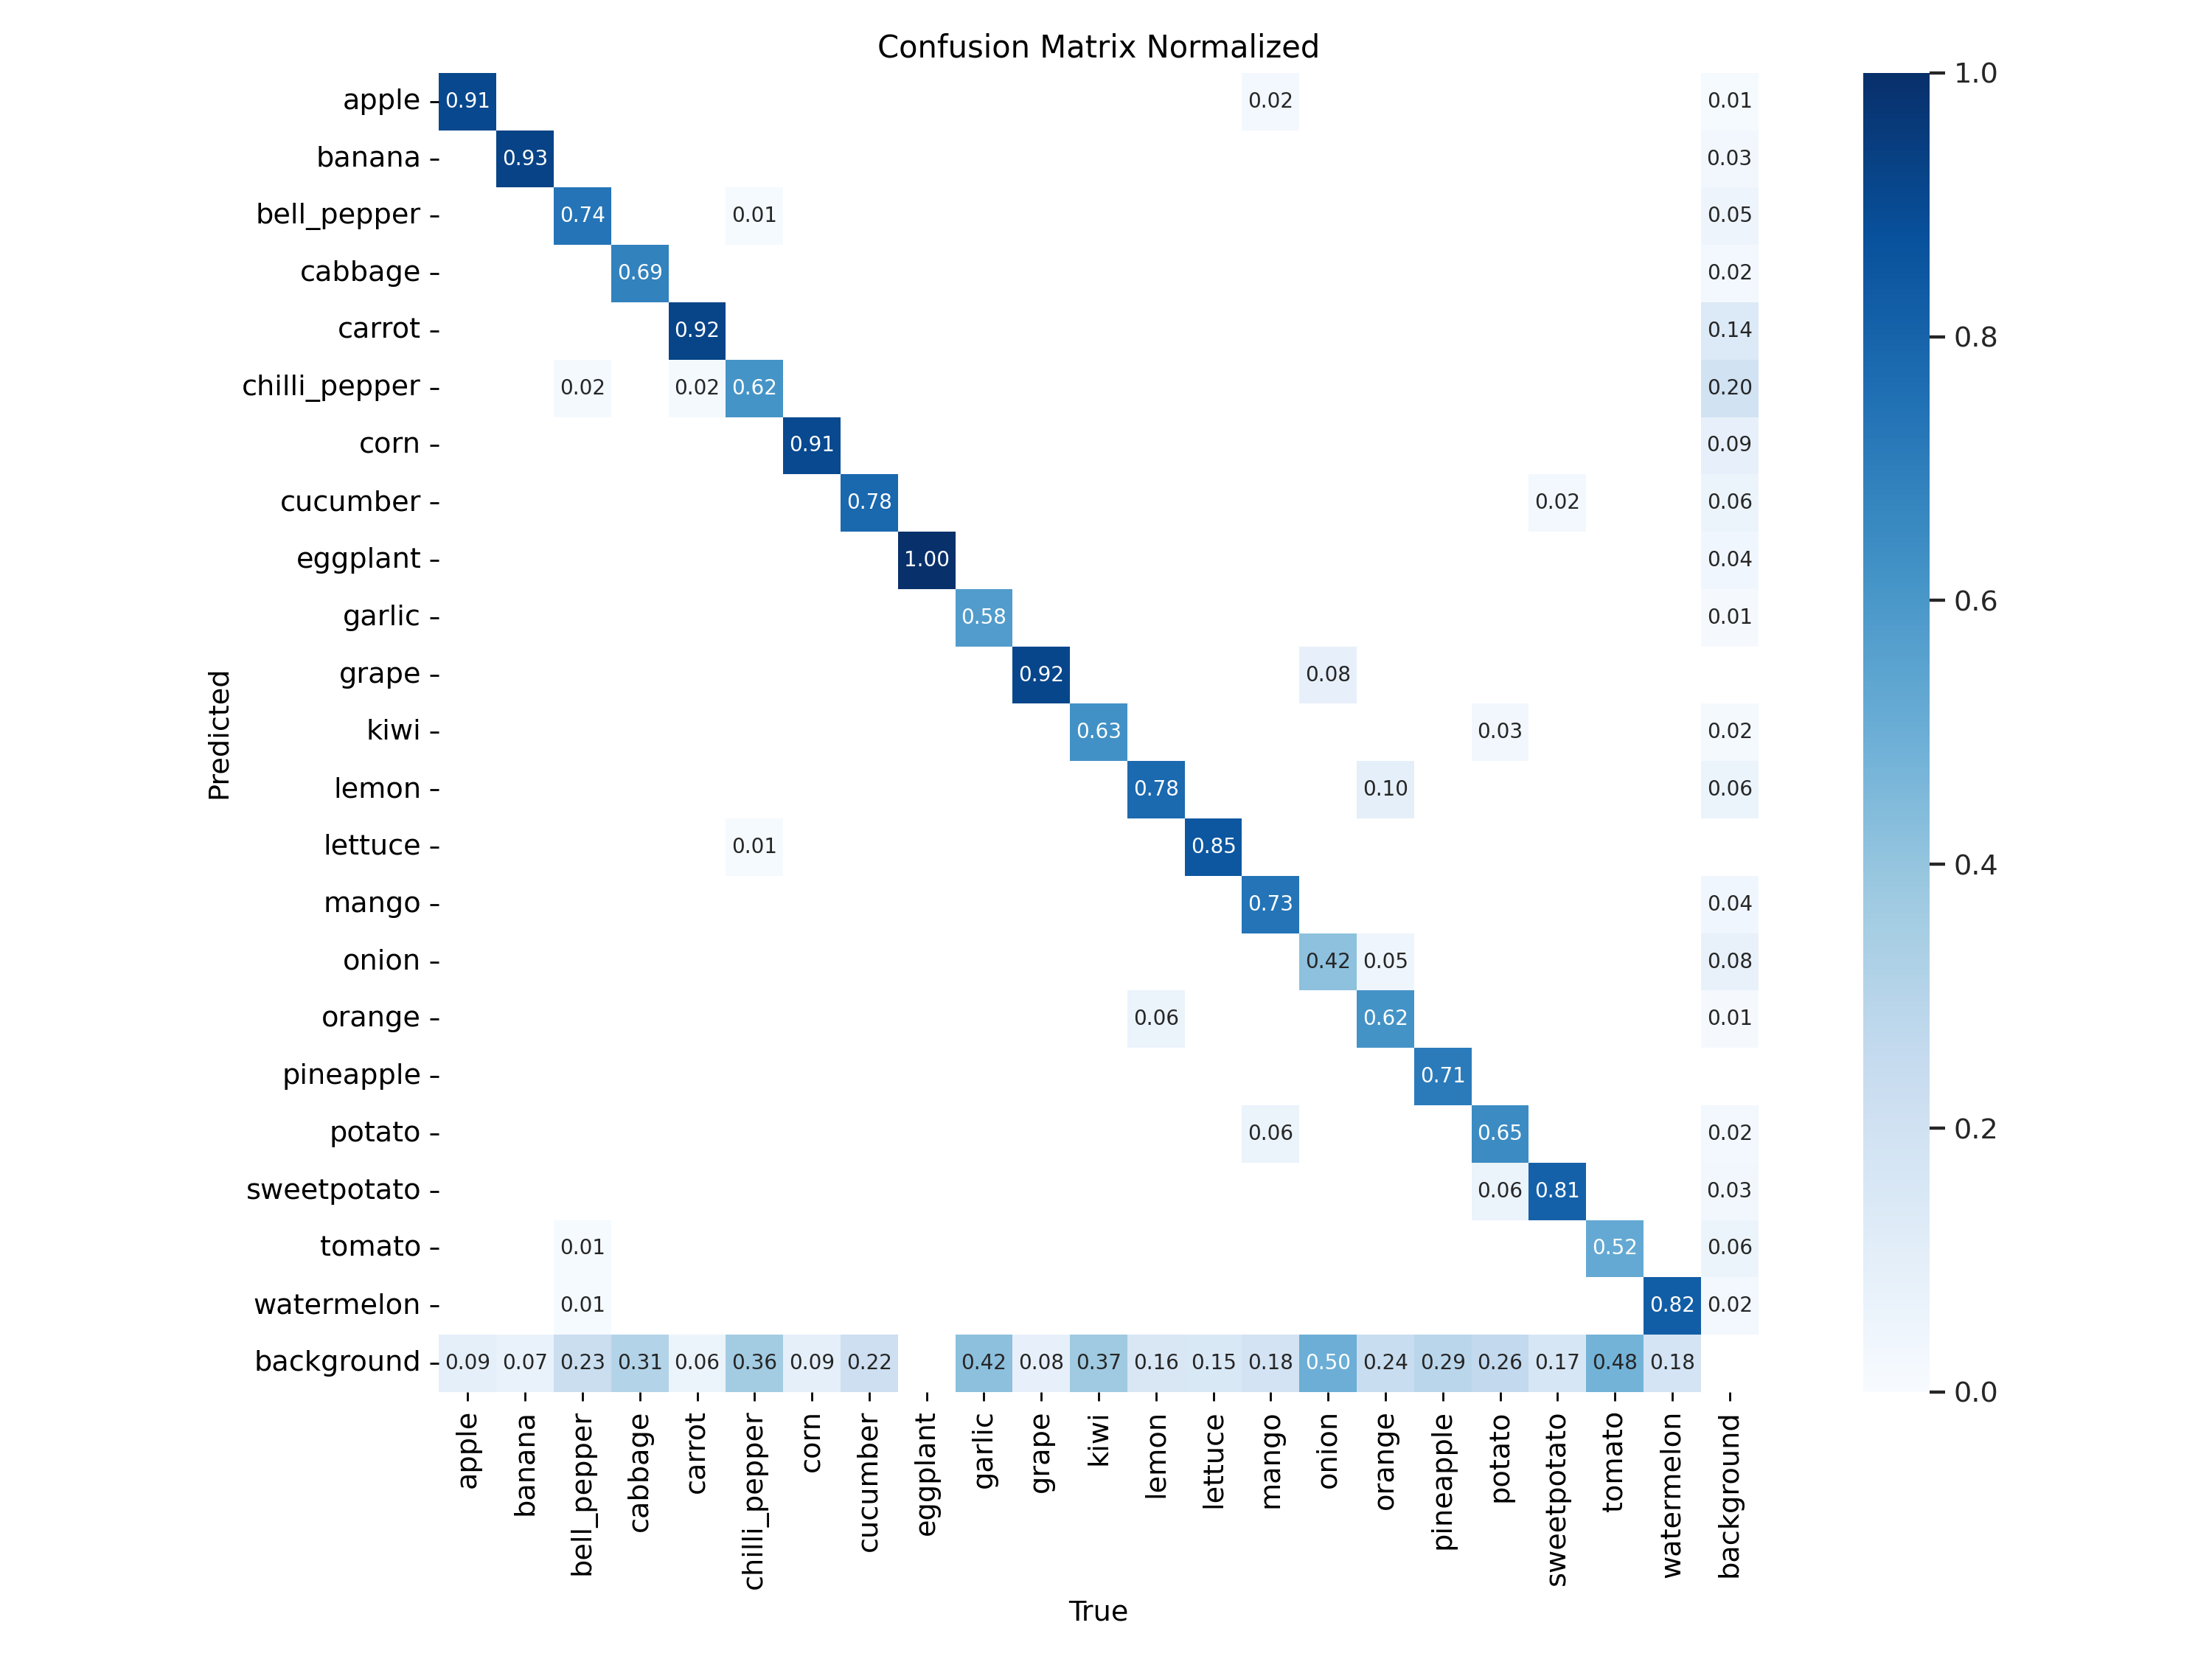
\includegraphics[width=0.8\linewidth]{../source/aws-img/yolov8/out/image/confusion_matrix_normalized.png}
    \caption{果实图像识别模型训练结果-标准化混淆矩阵图}
    \label{fig:confusion_matrix_normalized}
\end{figure}

从图\ref{fig:confusion_matrix_normalized}中的标准化混淆矩阵可以看出,模型在多个类别上表现出色。例如,apple(苹果)、banana(香蕉) 和 carrot(胡萝卜) 等类别的预测准确率都超过了 90\%。然而,某些类别的分类效果较差,chilli\_pepper(辣椒)的准确率为 62\%,并且容易被误分类为 corn(玉米) 或其他类别。总体来说,模型在多数类别上的表现良好,大部分类别的置信度都在 0.7 到 1.0 之间。

综上所述,训练出来的果实图像识别模型在精度与推理速度之间达到平衡,模型在多数类别上的识别效果表现良好。

对于称重数据的提交,下面根据压力测试的方法\cite{Zhu2017}来对其进行性能测试,通过测试软件 JMeter 模拟 HTTP 并发请求来统计各项性能指标:

1、测试环境:8 核 CPU, 8GB 内存 的 Docker 容器。

2、测试方式:启动称重相关服务,包含 Spring 应用服务、EMQX 集群以及MySQL 数据库服务,分别以并发数 100、200 和 500 对提交称重数据接口进行测试,Ramp-up Time(负载增长时间) 设为 30s,Hold Time(稳定负载时间)设为 35s。

3、测试结果:如图\ref{fig:jmeter-test-result}所示。

\begin{figure}[H]
    \centering
    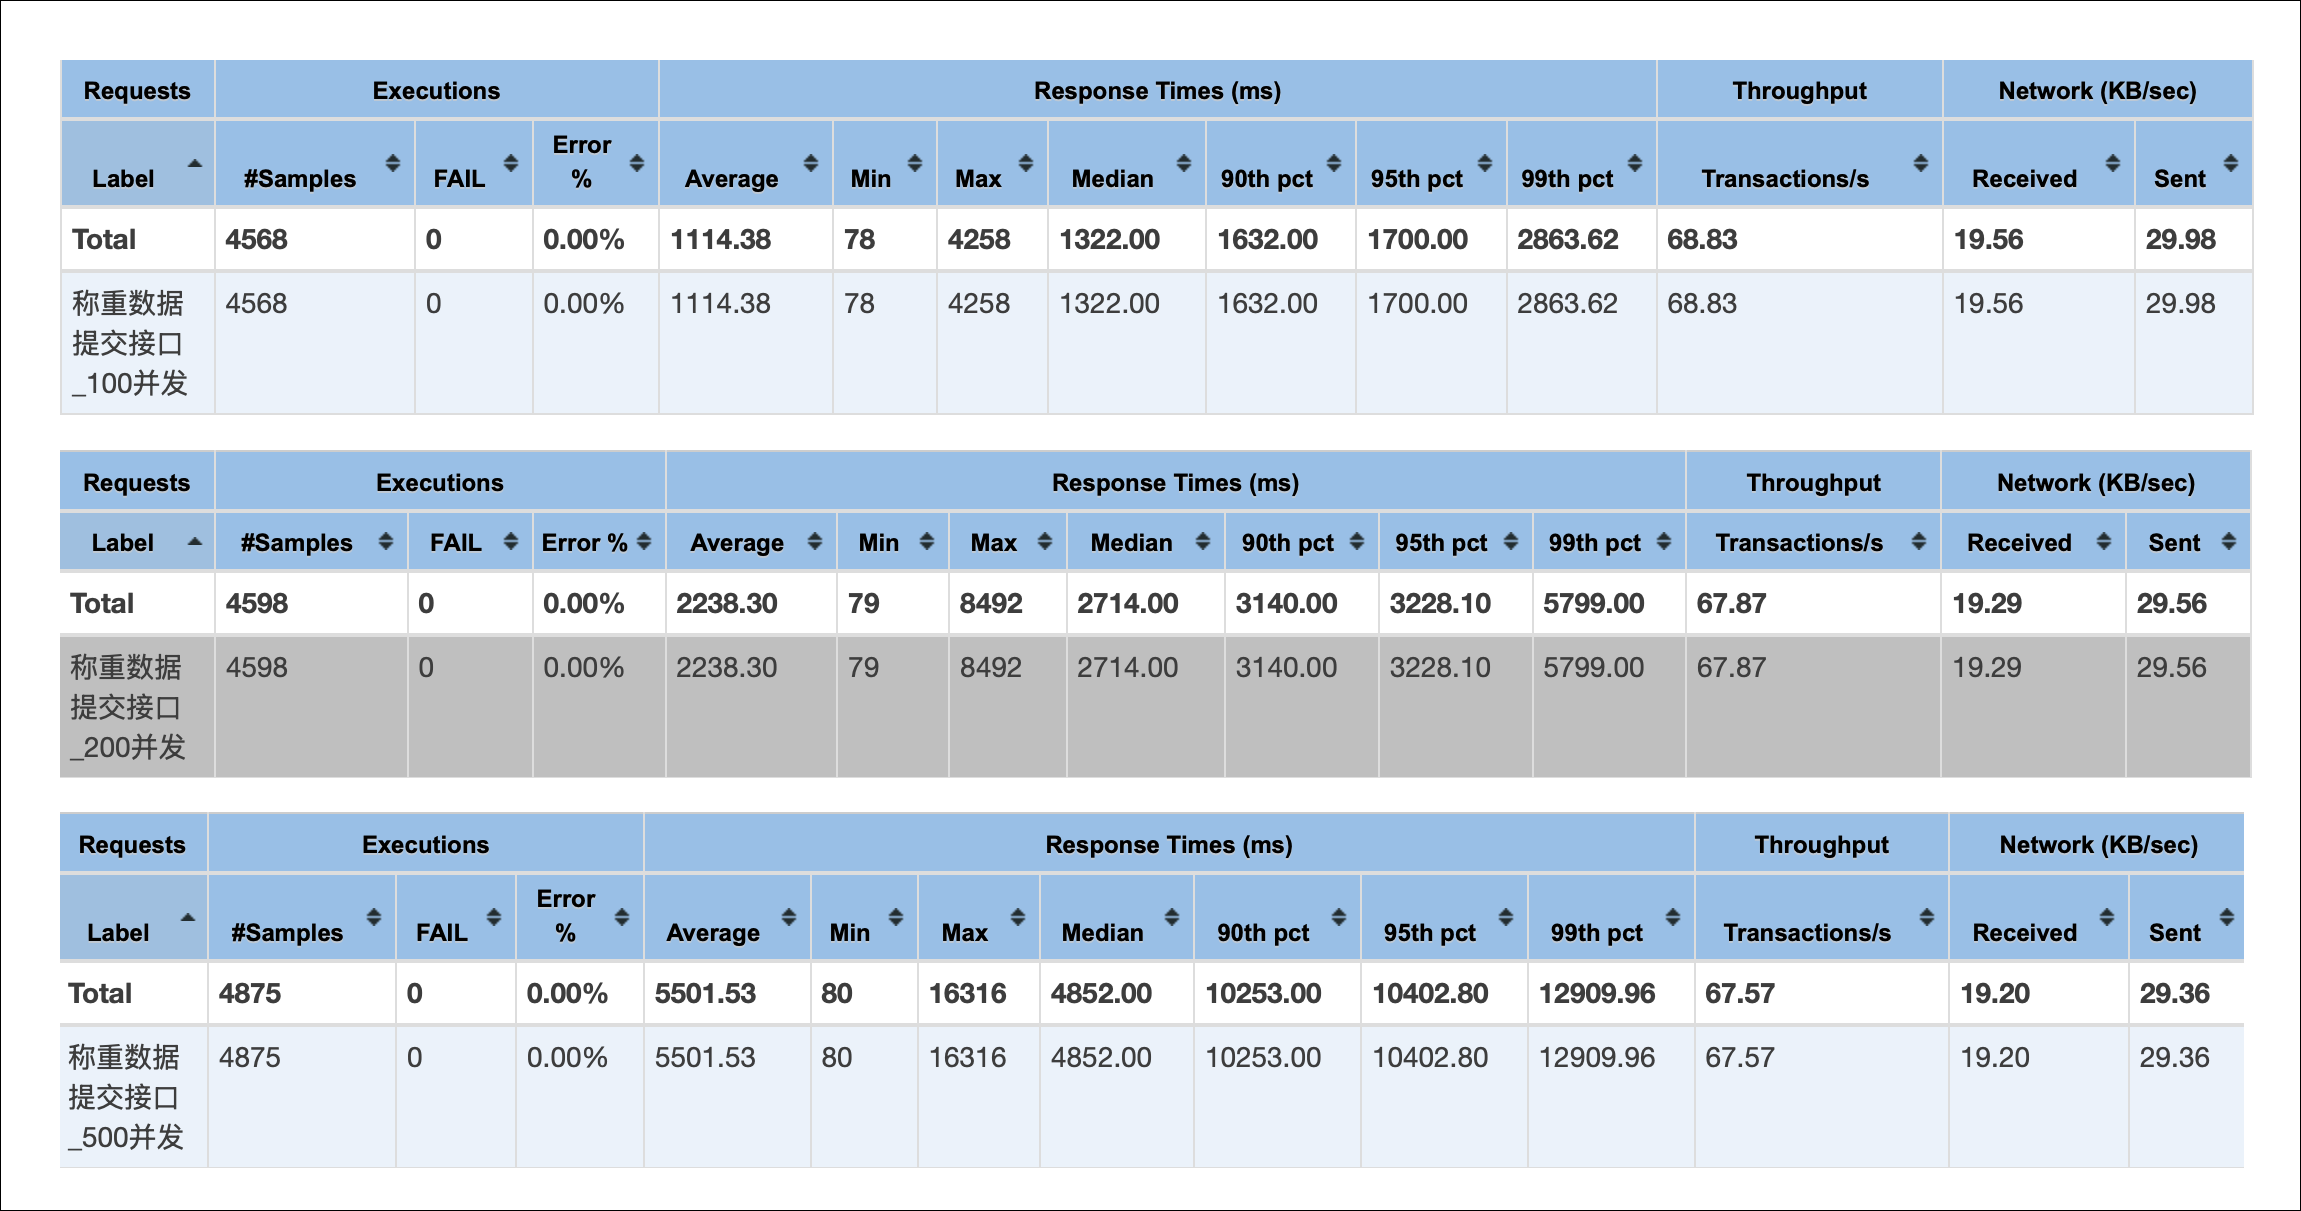
\includegraphics[width=0.8\linewidth]{../source/aws-test/result.png}
    \caption{核心接口的压力测试结果}
    \label{fig:jmeter-test-result}
\end{figure}

图\ref{fig:jmeter-test-result}从上至下显示了并发数为 100、200 和 500 下的压力测试结果表格,每个表格从左至右显示的条目分别是测试标题、样本数、失败数、错误率、平均响应时间、最小响应时间、最大响应时间、响应时间中位数、90\%响应时间、95\%响应时间、99\%响应时间、吞吐量、网络接收数据量、网络发送数据量。

在 100 并发下,软件性能表现较好,响应时间在 1 秒内,大部分请求能够在合理时间内完成,吞吐量也较为稳定。此时软件能够处理较高的负载;在 200 并发下,响应时间明显增加,超过了 2 秒,并且最大响应时间接近 9 秒。吞吐量略有下降,软件开始在中等负载下显现出性能下降的迹象。虽然软件能够处理较高并发,但开始显示出压力;在 500 并发下,性能显著下降,平均响应时间超过了 5 秒,最大响应时间接近 16 秒,90\% 的请求响应时间超过 10 秒。吞吐量保持不变或略微下降,说明软件在高负载下的性能有严重瓶颈,无法有效处理 500 并发请求。此时软件可能面临资源瓶颈。

从上述分析可以知道,在 8 核 CPU, 8GB 内存的硬件条件下,软件可以高效地处理超过 200 台电子秤的并发请求,适合于中小型农场的部署使用。如果将并发数提高到 500,可以考虑升级硬件资源。

\section{本章小结}

本章详细介绍了软件的实现与测试过程。首先对功能需求进行了全面测试,包括电子秤管理、果实管理、作业管理等核心功能模块,所有测试用例均通过验证。通过电子秤模拟器、管理后台界面和接口测试工具,验证了系统在不同协议下的数据传输、图像识别、统计分析等功能的正确性。

在非功能需求方面,重点测试了系统的性能和安全性。果实图像识别模型在精度与速度间取得平衡,识别准确率达到预期;压力测试表明系统可稳定支持200台电子秤并发工作,满足中小型农场需求。数据库加密和接口授权机制有效保障了数据安全。测试结果表明,系统各项指标均达到设计要求,为后续部署应用奠定了坚实基础。
